%\thispagestyle{empty}
\chapter{Численные эксперименты по моделированию нелинейных волновых движений и аномальных волн} \label{chapt3}

\section{Введение} \label{sect3_0}

Распространенным методом измерения морских волн является использование измерителей давления под водой или на морском дне. В частности, так работает американская система буев DART, предназначенная для регистрации цунами в открытом океане \cite{dart_Bernard}. Волны цунами являются достаточно длинными, так что вызываемое ими давление определяется известными формулами гидростатики. Учитывая к тому же, что такие буи установлены на больших глубинах, где ветровые волны уже не чувствуются, то задача восстановления смещения морской поверхности по вариациям придонного давления не вызывает особых затруднений. Если же датчики давления используются в мелком море, или при относительно небольшом погружении в воду, то они регистрируют колебания давления, связанные с волнами зыби и ветровыми волнами. Эти волны уже не являются длинными, так что давление в них не описывается гидростатической формулой. Такая ситуация, в частности, реализуется в условиях Охотского моря, где Институтом морской геологии и геофизики ДВО РАН \cite{firstResultsSakh_2009} и Специальным конструкторским бюро средств автоматизации морских исследований \cite{Zaits_Kuz_NGTU_2013} развернута система донных датчиков на глубинах от 10 до 20 м.

Восстановление колебаний морской поверхности, в частности волн зыби и ветровых волн, по данным регистраторов давления в общем случае является непростой задачей. Наиболее популярна в инженерной практике линейная теория волн на воде, определяющая связь между колебаниями придонного давления и морской поверхности \cite{Kuo_Chiu_1994} \cite{Zasl_Kras_2001} \cite{Tsai_Huang_2005} \cite{Baqueizo_Losada_1995}\cite{Huang_Tsai_2008}. Однако измерения показывают, что ошибка в предсказаниях параметров ветровых волн по данным регистраторов давления может достигать почти 20\% \cite{Bishop_Donelan_1987}. Имеющаяся разница обусловлена влиянием нелинейности морских волн, которая не учитывается в рамках линейной теории потенциального движения жидкости. Совсем недавно начались исследования этой проблемы с позиций полнонелинейной потенциальной теории волн на воде \cite{Esher_Schlurmann_2008} \cite{Constantin_Strauss_2010} \cite{Constantin_Esher_Hsu2011} \cite{Constantin_2012} \cite{Oliveras_2012} \cite{Deconink_2012}. Получаемые здесь уравнения представляют собой интегральные уравнения, весьма громоздкие и трудные для практического использования. Начаты также экспериментальные исследования связи между полем давления и морскими волнами в лотке \cite{Oliveras_2012}.

В данной главе исследуется связь колебаний морской поверхности и придонного давления в рамках численного решения уравнения Эйлера и а также в рамках слабо дисперсионных обобщений нелинейно теории мелкой воды.

Также в настоящей работе решается задача восстановления колебаний морской поверхности по данным регистратора давления решается в рамках слабо дисперсионных обобщений нелинейно теории мелкой воды в \cite{Green_1976}\cite{Zhel_Pel_1985} \cite{Fedotova_2008} \cite{Fedotova_2012}. Во втором параграфе приводятся основные уравнения модели Железняка--Пелиновского и выражение для давления в толще воды. В третьем параграфе описывается методика восстановления колебаний уровня моря по данным донных регистраторов. В четвертом параграфе даны результаты расчетов для условий Охотского моря. Полученные результаты суммированы в Заключении.




\section{Уравнения в конформных переменных с конечным дном}\label{sect3_1}
Рассмотрим нестационарное течение идеальной жидкости со свободной поверхностью в бассейне конечной глубины.

Пусть идеальная несжимаемая жидкость занимает область в плоскости $(x,y),$ ограниченную свободной поверхностью
\begin{gather*}
-\overline h<y<\eta(x,t),
\\
\\
-\infty<x<\infty,\quad t>0.
\end{gather*}
Также будем считать движение жидкости потенциальным, тогда:
$$
v(x,y,t)=\nabla\Phi(x,y,t),
$$
где $v(x,y,t)$~"--- поле скоростей в двумерной плоскости, $\Phi(x,y,t)$~"---
потенциал скоростей. Как следует из условия несжимаемости жидкости ${\rm div} v=0$, потенциал скоростей удовлетворяет уравнению Лапласа
$$
\Delta\Phi(x,y,t)=0.
$$
С этим уравнением связываются следующие граничные и начальные условия:
$$
(\eta_t+\Phi_x\eta_x-\Phi_y){|_{y=\eta(x,t)}}=0,
$$
$$
\left(\Phi_t+\dfrac{1}{2}|\nabla\Phi|^2+gy\right){|_{y=\eta(x,t)}}=0,
$$
$$
{\Phi_y}{|_{y=-\overline h}}=0, \eta{|_{t=0}}=\eta_0(x),
$$
$$
\Phi{|_{t=0}}=\Phi_0(x,y).
$$
Здесь $g$~"--- ускорение свободного падения.

Введем вспомогательную величину $\Psi(x,t)=\Phi(x,\eta(x,t),t),$ которая
является значением потенциала скоростей на свободной поверхности (см.
\cite{DiachZK1996}). Переменные $\eta$~и~$\Psi$ являются канонически сопряженными величинами, т.~е.
\begin{gather*}
\dfrac{\partial\eta}{\partial t}=\dfrac{\delta H}{\delta\Psi},
\\
\\
\dfrac{\partial\Psi}{\partial t}=\dfrac{\delta H}{\delta\eta},
\end{gather*}
где гамильтониан~$H$  совпадает с полной энергией жидкости
$H=T+U,$
\begin{gather*}
T=\dfrac{1}{2}\int\limits_{-\infty}^{\infty}dx\int\limits_{-\overline
h}^{\eta(x,t)} |\nabla\Phi|^2dy,
\\
\\
U=\dfrac{g}{2}\int\limits_{-\infty}^{\infty}\eta^2(x,t)dx.
\end{gather*}

В соответсвии с \cite{DiachZK1996} (Шамин)осуществим конформное преобразование области, которая занята жидкостью в плоскости $(x,y)$ в полупространство в
переменных $(u,v)$
\begin{gather*}
-\infty<u<\infty,\\
-h<v<0.
\end{gather*}
После операции отображения поверхность $\eta(x,t)$ можно представить в параметрическом виде
\begin{gather*}
y=y(u,t),\\
x=u+\tilde x(u,t).
\end{gather*}
Здесь $\tilde x(u,t)$ и $y(u,t)$ связаны следующим соотношением:
$$
y=R[\tilde x],
$$

где $R$ -- интегральный оператор вида

$$
R[f](u)=\dfrac{1}{2h}P.V.\int\limits_{-\infty}^{\infty}\dfrac{f(u')}{\sinh(\pi/2h(u'-u))}du'.
$$

Обратный к $R$ оператор $T$ имеет вид
$$
T[f](u)=\dfrac{1}{h}P.V.\int\limits_{-\infty}^{\infty}\dfrac{f(u')}{1-e^{-\pi/(h(u-u'))}}du'.
$$

Как показано в работе \cite{DiachZK1996}, переменные $y(u,t)$
и~$\Psi(u,t)$ полностью описывают движение жидкости и подчиняются
следующей системе интегродифференциальных уравнений, разрешенных
относительно производных по времени:
\begin{equation}\label{eq_z1}
y_t=-y_u
T\left[\dfrac{R[\Psi_u]}{J}\right]+x_u\dfrac{R[\Psi_u]}{J},
\end{equation}
\begin{equation}\label{eq_z2}
\Psi_t=-\dfrac{\Psi_u^2 - (R[\Psi_u])^2}{2J}
-T\left[\dfrac{R[\Psi_u]}{J}\right]\Psi_u - gy,
\end{equation}
где $J=x_u^2+y_u^2$~"--- якобиан отображения.

Уравнения~\eqref{eq_z1}--\eqref{eq_z2} в дальнейшем будут рассматриваться с
периодическими граничными условиями.

Пусть $u\in(0,2\pi),$ а функции $y,$ $\Psi$ представлены в виде:
\begin{gather*}\label{eq_kn}
y(u,t)=\sum\limits_{k=-\infty}^{\infty}y_k(t)e^{iku},
\\
\\
\Psi(u,t)=\sum\limits_{k=-\infty}^{\infty}\Psi_k(t)e^{iku}.
\end{gather*}
Операторы $R$ и $T$ в Фурье-представлении имеют простой вид:
$$
\begin{array}{ll}
y_k=R_k \tilde x_k, & R_k=i\tanh kh, \\
\\
\tilde x_k=T_ky_k, & T_k=-i\coth kh. \\
\end{array}
$$
Операция дифференцирования по переменной $u$ в Фурье-представлении
имеет вид:
$$
D_k=ik.
$$

\section{Исследование влияния нелинейности морских волн на характеристики вариаций придонного давления с помощью численных экспериментов} \label{sect3_2}
\subsection{Расчет давления на глубине идеальной жидкости при использовании конформного отображения}
Для оценки давления на глубине в полнонелинейном случае рассмотрим подход к описанию динамики свободной жидкости конечной глубины, исходя из вариационного принципа и при использовании конформного отображения, описанный в работе \cite{DiachZK1996}. Неявные уравнения для потенциала и конформного отображения в полосу возникают как уравнения Эйлера-Лагранжа.
Для оценки давления на дне рассмотрим уравнение Бернулли:
\begin{equation}\label{eq:bern}
p_{bottom}=\rho gh-\rho \frac{\partial\Phi_{bottom}}{\partial t}
\end{equation}
где  $\Phi_{bottom}$ - потенциал на дне, h – глубина, $\rho$ - плотность жидкости. Следуя \eqref{eq:bern} основную проблему составляет нахождение потенциала на дне, поскольку все остальные члены уравнения известны.

В работе \cite{DiachZK1996} показано, что при конформном преобразовании потенциал   остается гармонической функцией в полосе, т.е. удовлетворяет уравнению Лапласа.
\begin{equation}\label{eq:laplas}
\frac{\partial^2\Phi}{\partial u^2}+\frac{\partial^2\Phi}{\partial v^2} = 0
\end{equation}
с граничными условиями
\begin{equation}\label{eq:laplasGranUsl}
\frac{\partial\Phi}{\partial v}\mid_{v=-h}=0, \Phi\mid_{v=0}=\Psi(u,t),
\end{equation}
где $\Psi(u,t)$ потенциал на свободной поверхности

Также в работе \cite{DiachZK1996} показано, что существует интегральный оператор $\hat{R}$ вида:
\begin{equation}\label{eq:intR}
\hat{R}f(u)=\frac{1}{2\pi}P.V.\int\limits_{-\infty}^{+\infty}\frac{f(u')}{sh(\pi/2h(u'-u))}du'
\end{equation}
в Фурье-представлении он локален и записывается существенно проще:
\begin{equation}\label{eq:intR_fourie}
R_k=ith(kh)
\end{equation}
С помощью оператора $\hat{R}$  для любой действительной достаточно гладкой функции $\phi(w)$ , которая задана на действительной оси и затухает на бесконечности $u\rightarrow\infty$, можно построить комплексный потенциал $\Theta(w=u+iv,t)$, который будет аналитически продолжим в полосу $-h\leq v\leq0$, т.е. на всю толщину жидкости:
\begin{equation}\label{eq:teorComplPotential}
\theta=\phi+i\hat{R}\phi
\end{equation}
Применяя процедуру \eqref{eq:teorComplPotential} к потенциалу на свободной поверхности  $\Psi(u,t)$, приходим к комплексному потенциалу, который на действительной оси равен:
\begin{equation}\label{eq:myComplPotential}
\Theta(w,t)=\Psi(u,t)+i\hat{R}\Psi(u,t)
\end{equation}

Аналитически продолжимый $\Theta(w,t)$ комплексный потенциал   можно записать в виде ряда Фурье:

\begin{equation}\label{eq:MainResult}
\begin{split}
\Theta(w,t) = \sum\limits_{k=-\infty}^{\infty}\varphi_ke^{ikw}+i\sum\limits_{k=-\infty}^{\infty}i\th(kh)\varphi_ke^{ikw}=\\
&=\sum\limits_{k=-\infty}^{\infty}\varphi_ke^{ikw}-\sum\limits_{k=-\infty}^{\infty}\th(kh)\varphi_ke^{ikw}=\\
&=\sum\limits_{k=-\infty}^{\infty}(1-\th(kh))\varphi_ke^{ikw}
\end{split}
\end{equation}
где  $\varphi(k)$ - коэффициенты ряда Фурье для потенциала на поверхности.
Т.к.  функция $\Theta(w,t)$  аналитически продолжима, то можем составить комплексный потенциал на определенной глубине $v$, т.е. $w=u+iv$ :

\begin{equation}\label{eq:MainResult_1}
\begin{split}
\Theta(u+iv,t) = \sum\limits_{k=-\infty}^{\infty}(1-\th(kh))\varphi_ke^{ik(u+iv)}=\\
&=\sum\limits_{k=-\infty}^{\infty}(1-\th(kh))\varphi_ke^{iku}e^{ik(iz)}=\\
&=\sum\limits_{k=-\infty}^{\infty}(1-\th(kh))\varphi_ke^{iku}e^{-kv}
\end{split}
\end{equation}


Таким образом потенциал скоростей на дне ($v=-h$) будет равен:

\begin{equation}\label{eq:PotentialBottom}
\Phi_{bottom}(u,t)=Re(\Theta(u-ih,t))=Re[\sum\limits_{k=-\infty}^{\infty}(1-\th(kh))e^{kh}\varphi_ke^{iku}]
\end{equation}

\subsection{Численные эксперименты }

Рассмотрим серию численных экспериментов по решению полнонелинейных уравнений, записанных в конформных переменных, для плоского нестационарного потенциального течения идеальной жидкости со свободной поверхностью и конечной глубиной. По пространственным переменным рассматривались $2\pi$ периодические граничные условия. Начальные условия выбираются в соответствие с теми, что наблюдались в Охотском море в натурных экспериментах. Глубина бассейна бралась 14 метров, длина начальной волны  составляет 150 метров, амплитуды волн при этом варьировались от 3 см до 3.58 м, соответственно, крутизна при этом варьировалась от ka=0.0012 до ka=0.15.  При этом виртуальный волнограф, записывающий придонное давление и смещение поверхности, устанавливался в точке на донной поверхности.

Опишем подробно остальные параметры численных расчетов:
\begin{itemize}
  \item Глубина бассейна - h=14 m
  \item Длина области – $L_{area}=150$m
  \item Длина начальной волны - $\lambda=150$ m
  \item Ускорение свободного падения - g=9.81 $m/s^2$
  \item Дискретизация волнограммы, записываемой в одной точке профиля 10Hz;
\end{itemize}

Таким образом в начальный момент времени форма волны была
\begin{equation}\label{eq:beginWave}
\eta(x,t=0)=Acos(x)
\end{equation}
а потенциал на свободной поверхности, в соответствие с линейной теорией, в начальный момент времени задавался как:
\begin{equation}\label{eq:beginPotential}
\psi(x,t=0)=-A\sqrt{\frac{G}{h}}sin(x)
\end{equation}
здесь x – безразмерная пространственная переменная $x=[0,2\pi]$, A – безразмерная нормированная амплитуда колебаний, G - безразмерное ускорение свободного падения. Нормировка при этом вводится подобно описанной в разделе \ref{sect_linTheory_norming} Главы 1.
%Расписать подробнее про нормировку
\begin{equation}\label{eq:norming}
\beta_{norm}=\frac{L_{area}}{2\pi}, A=\frac{A_{phys}}{\beta_{norm}}
\end{equation}
где $\beta_{norm}$ - коэффициент нормировки,  $L_{area}$ - длина профиля выраженная в метрах(в нашем случае равна 150 м), $A_{phys}$ - амплитуда колебаний выраженная в метрах (в нашем случае задается в диапазоне от 3.58 м до 0.03 м).

%Подобным образом задаются остальные физические параметры, так, например безразмерное ускорение свободного падения, задается следующим образом:

Нормирование времени, при этом, определяется следующей формулой
\begin{equation}\label{eq:normingG}
t = \sqrt{\frac{\beta_{norm}}{g}}t.
%G=\frac{9.81}{\beta_{norm}} %тут другая нормировка должна быть через время!
\end{equation}

На рис.\ref{img:beginWave} представлена форма волны в начальный момент времени, стрелкой отмечено положение виртуального волнографа на рассматриваемой области. Волнограф находится на середине исследуемого профиля на расстоянии 75 метров от границ.
\begin{figure} [h]
  \center
  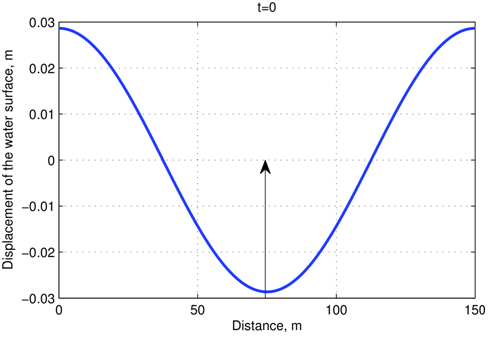
\includegraphics [scale=1] {beginWave.png}
  \caption{Профиль поверхности в начальный момент времени, линией отмечено положение виртуального волнографа}
  \label{img:beginWave}
\end{figure}
\FloatBarrier

Подробно рассмотрим эксперимент с наименьшей амплитудой колебаний и крутизной волны A=2.86см $ka=2\pi A/\lambda=20.0286/150=0.0012$. Профиль начальной волны представлен на рис.\ref{img:beginWave}.
Далее найдем численное решения полнонелинейных уравнений для плоского нестационарного потенциального течения идеальной жидкости со свободной поверхностью и конечной глубиной.
На рис.\ref{img:beginWavegramm} представлена запись виртуального волнографа, который ведет регистрацию с дискретностью 10Нz. Как видно из этой волнограммы развитие волны происходит практически без изменений, и амплитуда колебаний не меняется со временем, следовательно можно сказать что рассматриваемый процесс является линейным.
\begin{figure} [h]
  \center
  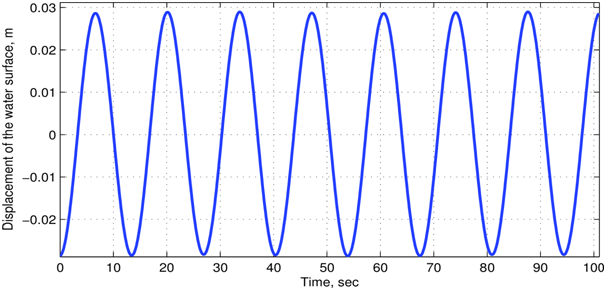
\includegraphics [scale=1] {beginWavegramm.png}
  \caption{Волнограмма колебания поверхности в точке для начальной волны, линией отмечено положение виртуального волнографа}
  \label{img:beginWavegramm}
\end{figure}
\FloatBarrier
В данном случае параметр характеризующий тип дисперсионного соотношения равен $kh=2\pi h/L_{area}=2\pi14/150=0.58$. В случае когда $kh\ll1$ можно пользоваться дисперсионным соотношением мелкой воды:
\begin{equation}\label{eq:smallwater}
w=k\sqrt{gh}
\end{equation}
В нашем случае параметр $kh$ не значительно меньше 1, но тем не менее меньше. Поэтому можно использовать дисперсионное соотношение \eqref{eq:smallwater} и как следствие оценить период волн по формуле:
$$
T=\frac{L_{area}}{\sqrt{gh}}=\frac{150}{\sqrt{14g}}=12.8
$$
Этот период колебаний, рассчитанный по дисперсионному соотношению мелкой воды, совпадает с периодом колебаний, записанных виртуальным волнографом.
\subsection{Сравнительный анализ придонного давления, рассчитанного с использованием линейной и полнонелинейной теории}
Рассмотрим давление на дне рассчитанное с помощью двух формул: линейной и нелинейной теории.
\begin{equation}\label{eq:pressFullLin_Nonlin}
P_{nonlin}(t)=\rho gh-\rho\frac{\partial\Phi_{bottom}}{\partial t},
P_{lin}=R^{-1}(\eta(t)+h)
\end{equation}

где h – глубина бассейна,  $\rho$ - плотность жидкости, $\eta(t)$ - смещение свободной поверхности в разные моменты времени, $\Phi_{bottom}$ - потенциал на дне, R – функция-оператор, которая в соответствие с линейной теорией преобразует придонное давление в смещение поверхности, соответственно $R^{-1}$ - обратная к ней.

Далее для удобства сравнения будем рассматривать давление без постоянной гидростатической части  $\rho gh$, т.е. далее будем считать что:

\begin{equation}\label{eq:pressNonlin}
P_{nonlin}(t)=-\rho\frac{\partial\Phi_{bottom}}{\partial t},
\end{equation}

\begin{equation}\label{eq:pressLin}
P_{lin}=R^{-1}(\eta(t))
\end{equation}


Далее на рис.\ref{img:compareLinTheory} представлено сравнение давления на дне, полученного в результате численного решения полнонелинейных уравнений, и рассчитанного из смещения поверхности по формулам линейной теории.

\begin{figure} [h]
  \center
  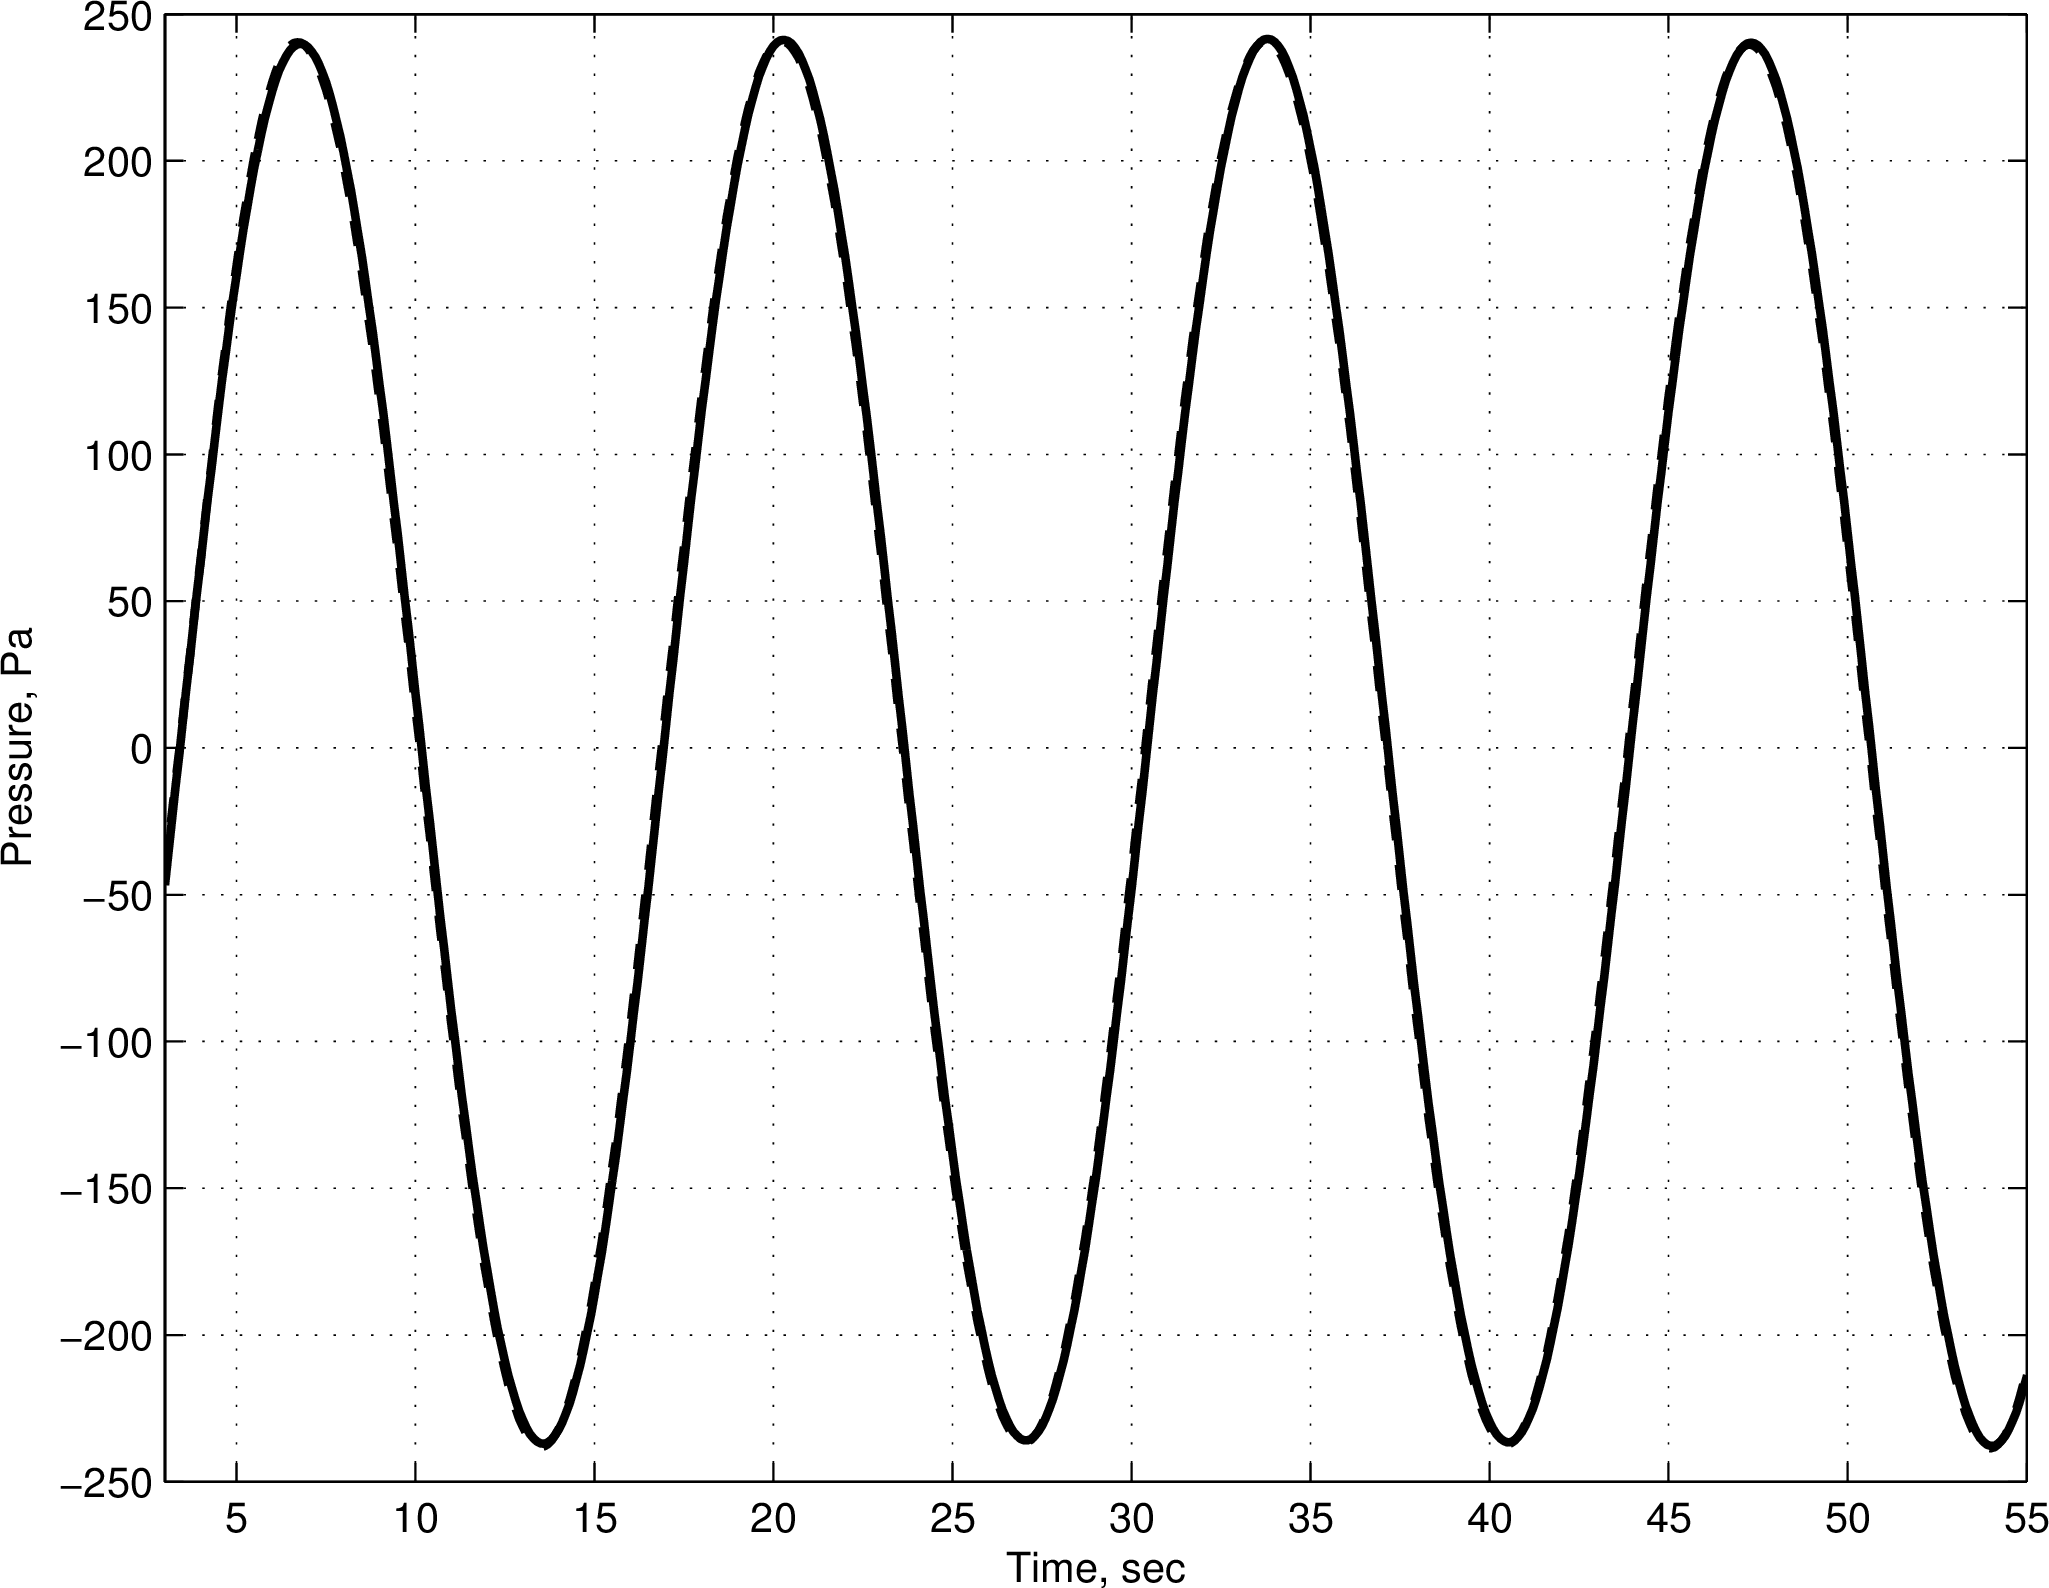
\includegraphics [scale=1] {compareLinTheory.png}
  \caption{График пульсаций придонного давления, рассчитанного по нелинейной теории (сплошная линия)и по линейной теории (пунктирная линия) для начальной волны с крутизной k=0.0012 и амплитудой A=3см}
  \label{img:compareLinTheory}
\end{figure}
\FloatBarrier

Из рис.\ref{img:compareLinTheory} видно, что давление на дне, раcсчитанное с помощью линейной и нелинейной теорий практически полностью совпадает, что говорит о линейности протекающего процесса.

Рассмотрим относительное отклонение результатов расчетов по линейной и нелинейной теории, для этого будем использовать следующую формулу:

\begin{equation}\label{eq:relatError}
\delta(t)=\frac{P_{lin}(t)-P_{nonlin}(t)}{P_{max}-P_{min}}
\end{equation}

где $P_{nonlin}(t)$ - вариации придонного давления, рассчитанные по формуле \eqref{eq:pressNonlin}, получаемая из нелинейного уравнения Эйлера в конформных переменных, $P_{lin}(t)$ - вариации придонного давления, рассчитанные по формуле линейной теории \eqref{eq:pressLin}, $P_{max}, P_{min}$ - максимальное и минимальное значения давления рассчитанного по формуле \eqref{eq:pressNonlin}.

Таким образом $\delta(t)$ - безразмерная величина, показывающая отклонение в зависимости от высоты колебаний нелинейного давления.

\begin{figure} [h]
  \center
  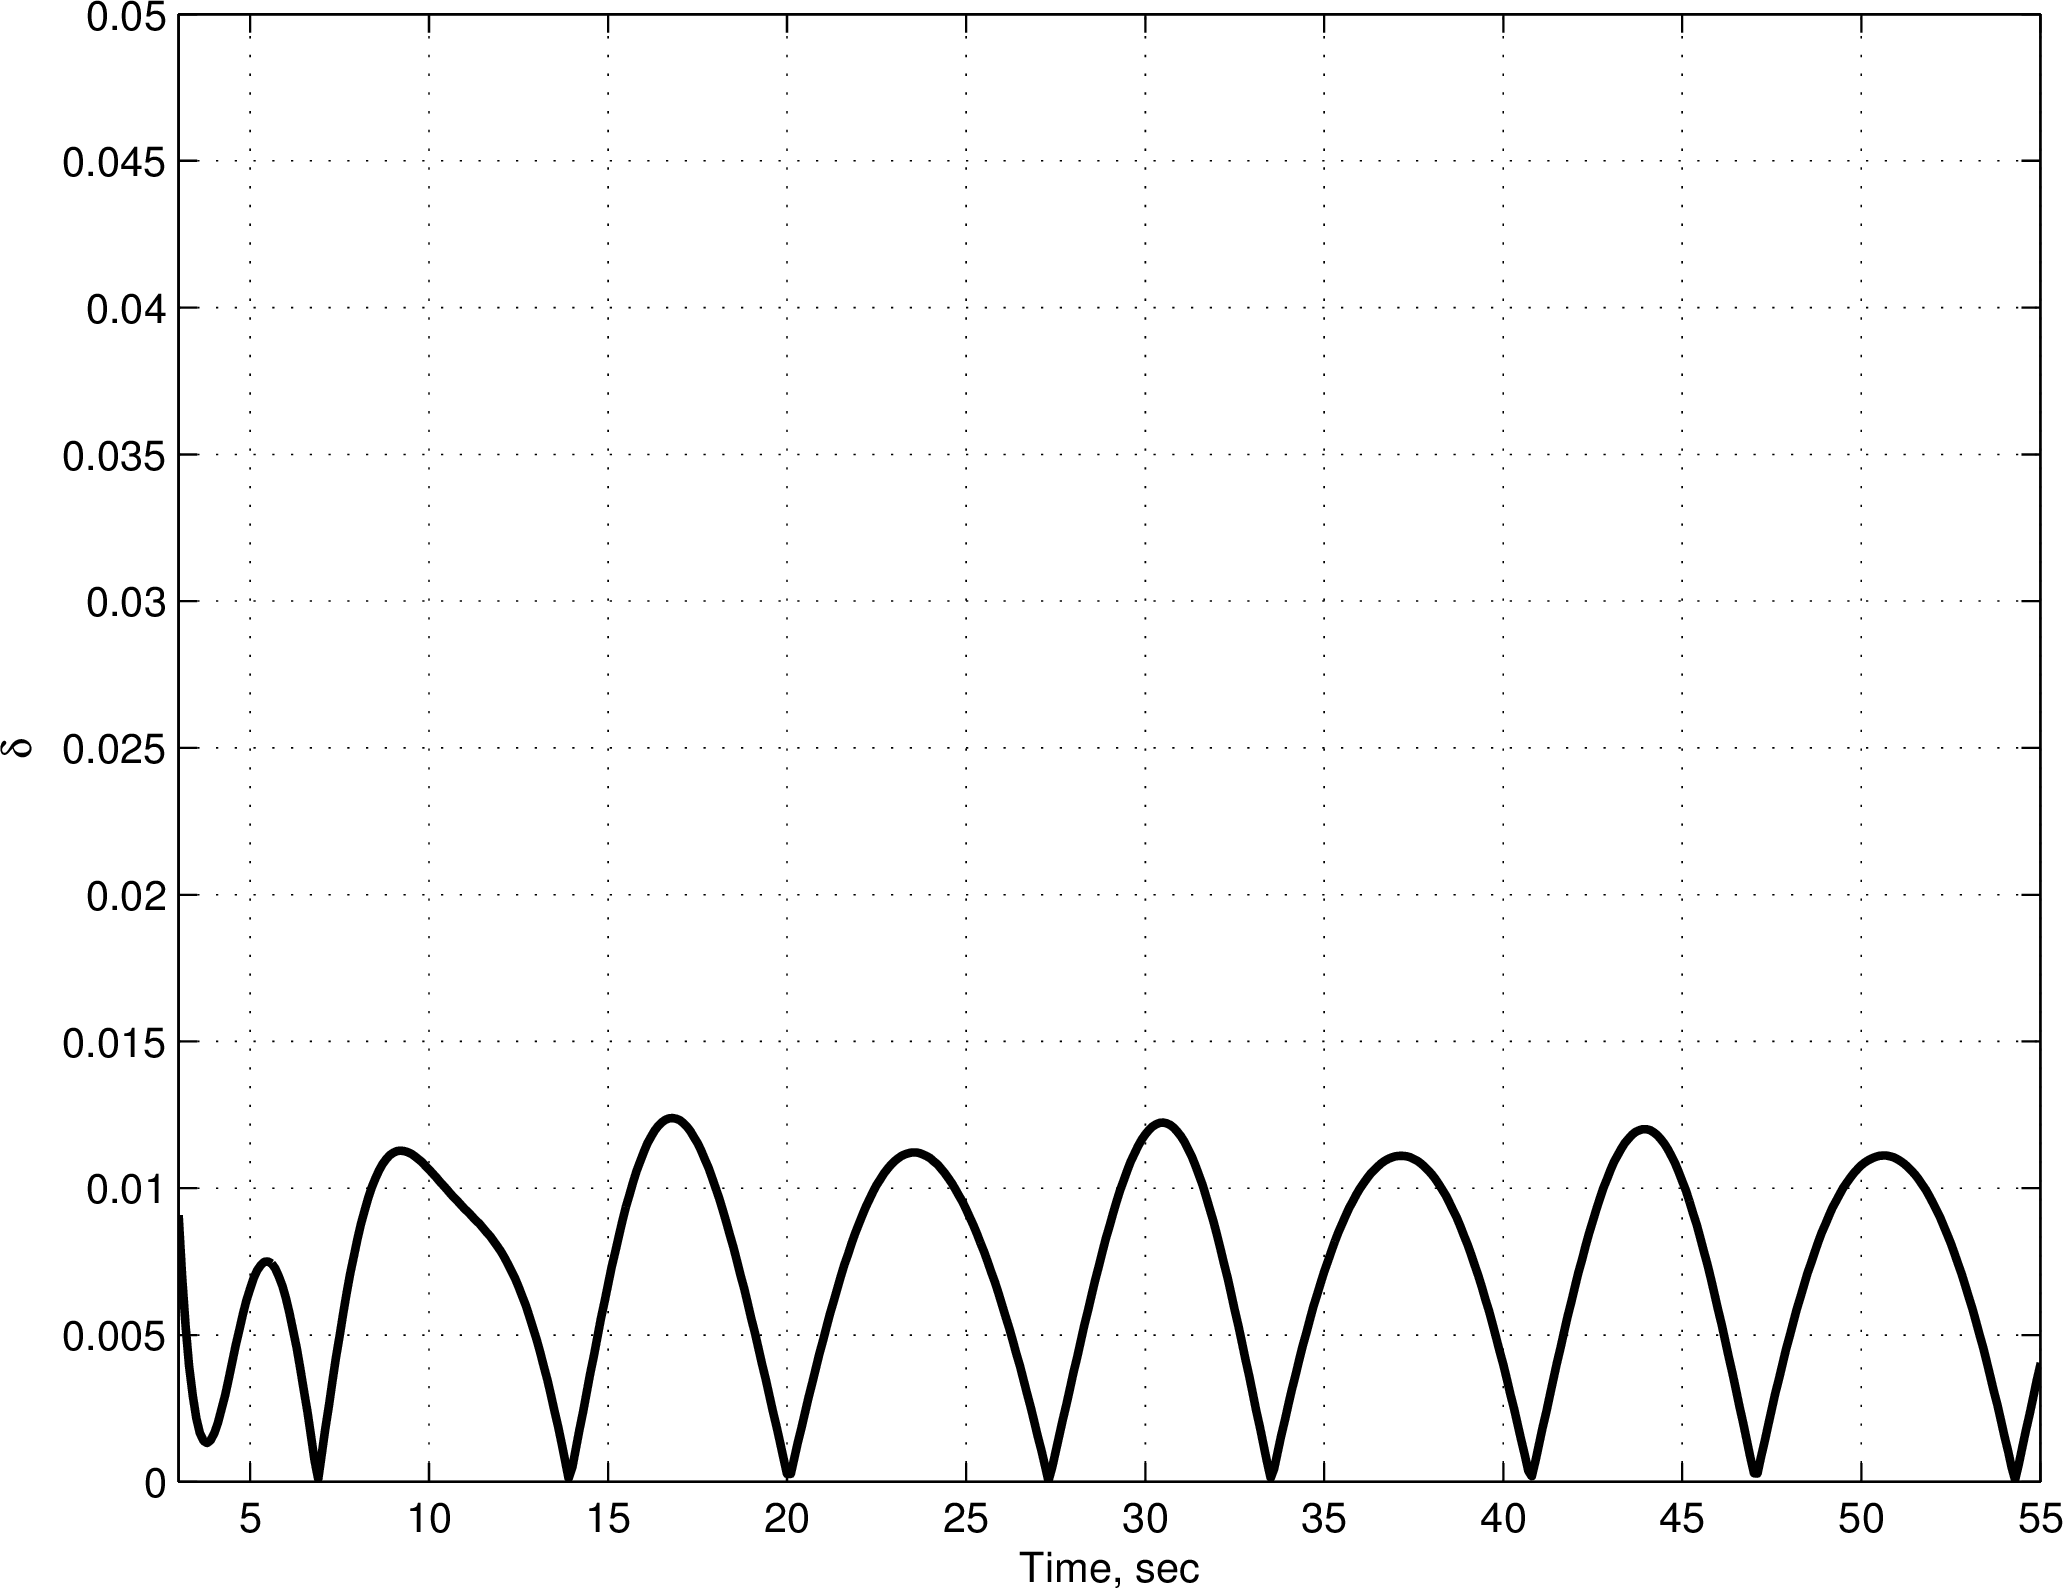
\includegraphics [width=0.7\linewidth] {relErrorLin.png}
  \caption{Модуль относительного отклонения придонного давления рассчитанного по линейной и нелинейной формулам для начальной волны с крутизной k=0.0012 и амплитудой A=3см}
  \label{img:relErrorLin}
\end{figure}
\FloatBarrier

На рис.\ref{img:relErrorLin} представлен график колебания величины $|\delta(t)|$ для случая линейного процесса (А=3 см). Как видно среднее относительные отклонение давлений, рассчитанных с помощью линейной и нелинейной теории, составляет около 0.7\%, а максимум составляет 1.3\% даже при очень малой амплитуде. Такое отличие не может быть связано с численными ошибками в методиках расчета, так как, кроме аппроксимации Ханта \cite{hunt}, в них не используется никаких приближений, в том числе и при решении полнонелинейных уравнений. Более вероятно, что такое отличие связано с присутствием малой нелинейности.

Таким образом показано, что в случае линейного процесса результаты расчетов по методикам основанным на линейной и нелинейной теории совпадают.

\subsection{Характеристики давления при сильнонелинейных процессах}

Рассмотрим существенно более нелинейный процесс с начальной волной амплитудой 1.9 метра и длиной 150 метров, соответственно крутизна начальной волны будет ka=0.08.

\begin{figure} [h]
  \center
  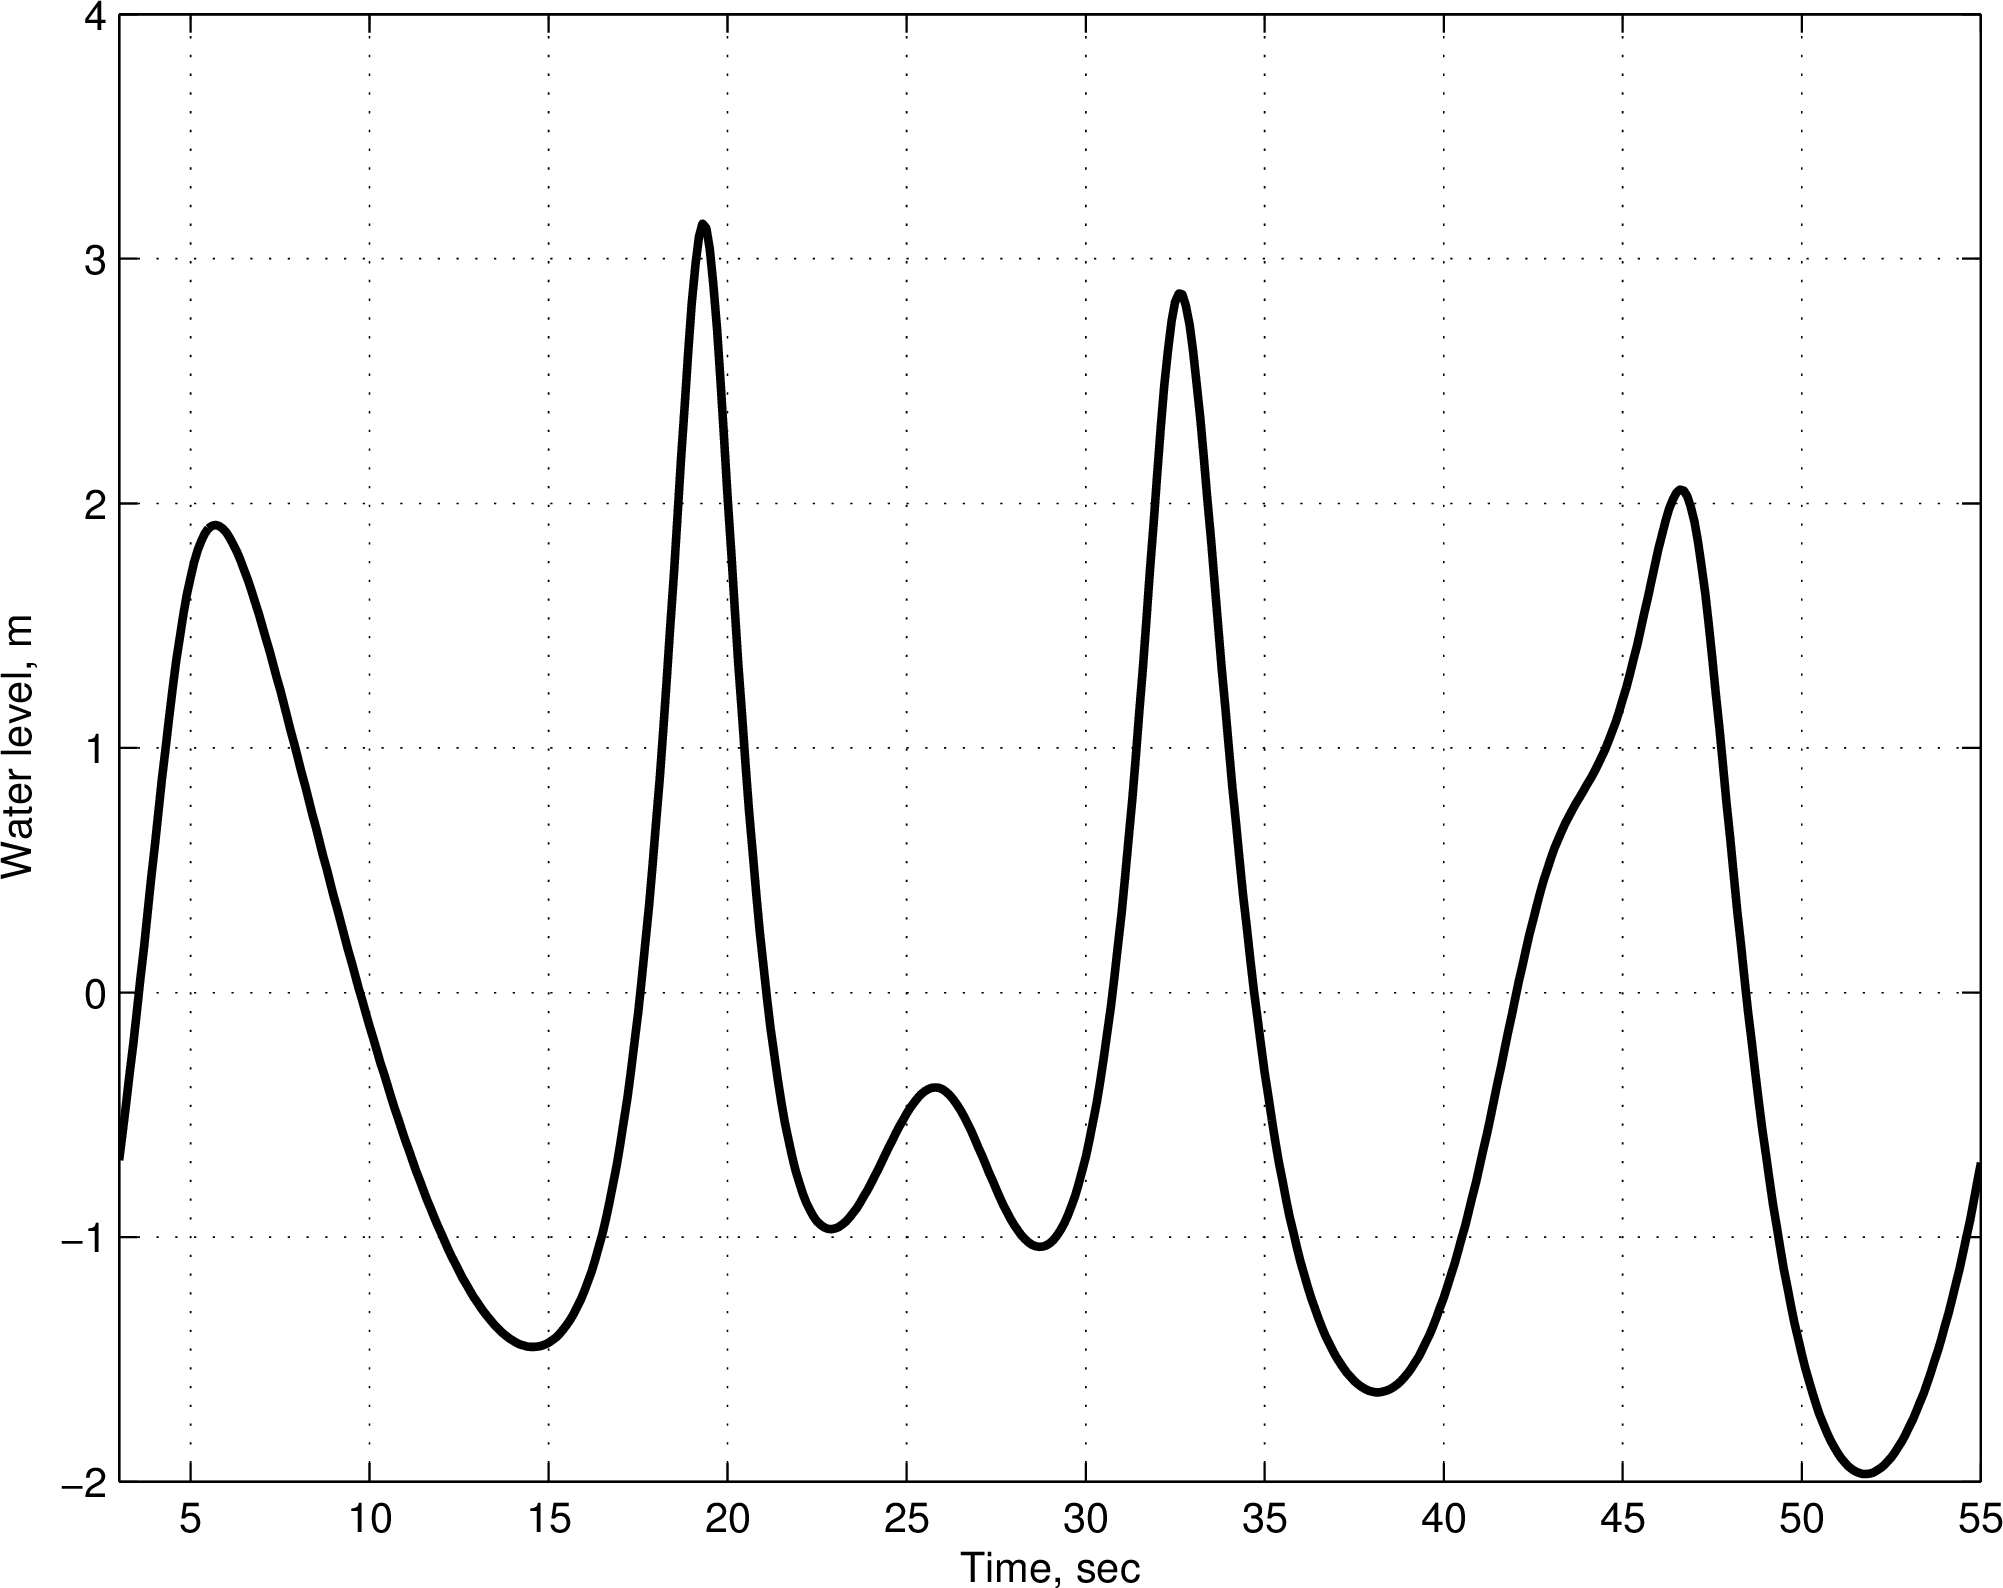
\includegraphics [scale=0.9] {wavegrammNonlin.png}
  \caption{Волнограмма колебания поверхности в точке для начальной волны c амплитудой A=1.9 м и крутизной k=0.08}
  \label{img:wavegrammNonlin}
\end{figure}
\FloatBarrier

На рис.\ref{img:wavegrammNonlin} представлена волнограмма, записанная виртуальным волнографом в точке,  подробно описанным выше. На записи видна эволюция поверхностной волны, достаточно быстро она становится нерегулярной, а после 60 секунды решение разрушается. При этом процессе так же стоит отметить, несколько моментов которые отмечаются в том числе и в других численных экспериментах:
\begin{enumerate}
  \item Заострение гребней и уплощение подошвы, т.е. форма волн становится похожей на волны Стокса,
  \item Сильная нерегулярность высот индивидуальных волн.
\end{enumerate}
Подобные эффекты проявляются тем меньше, чем меньше крутизна волны, задаваемой в начальный момент времени.

На рис.\ref{img:compareNonlinTheory} представлено сравнение пульсаций давления у дна, рассчитанного  по нелинейной формуле и по формулам линейной теории для крутизны 0.08, как видно из этого рисунка, линейная теория недооценивает максимумы давления и переоценивает минимумы.

\begin{figure} [h]
  \center
  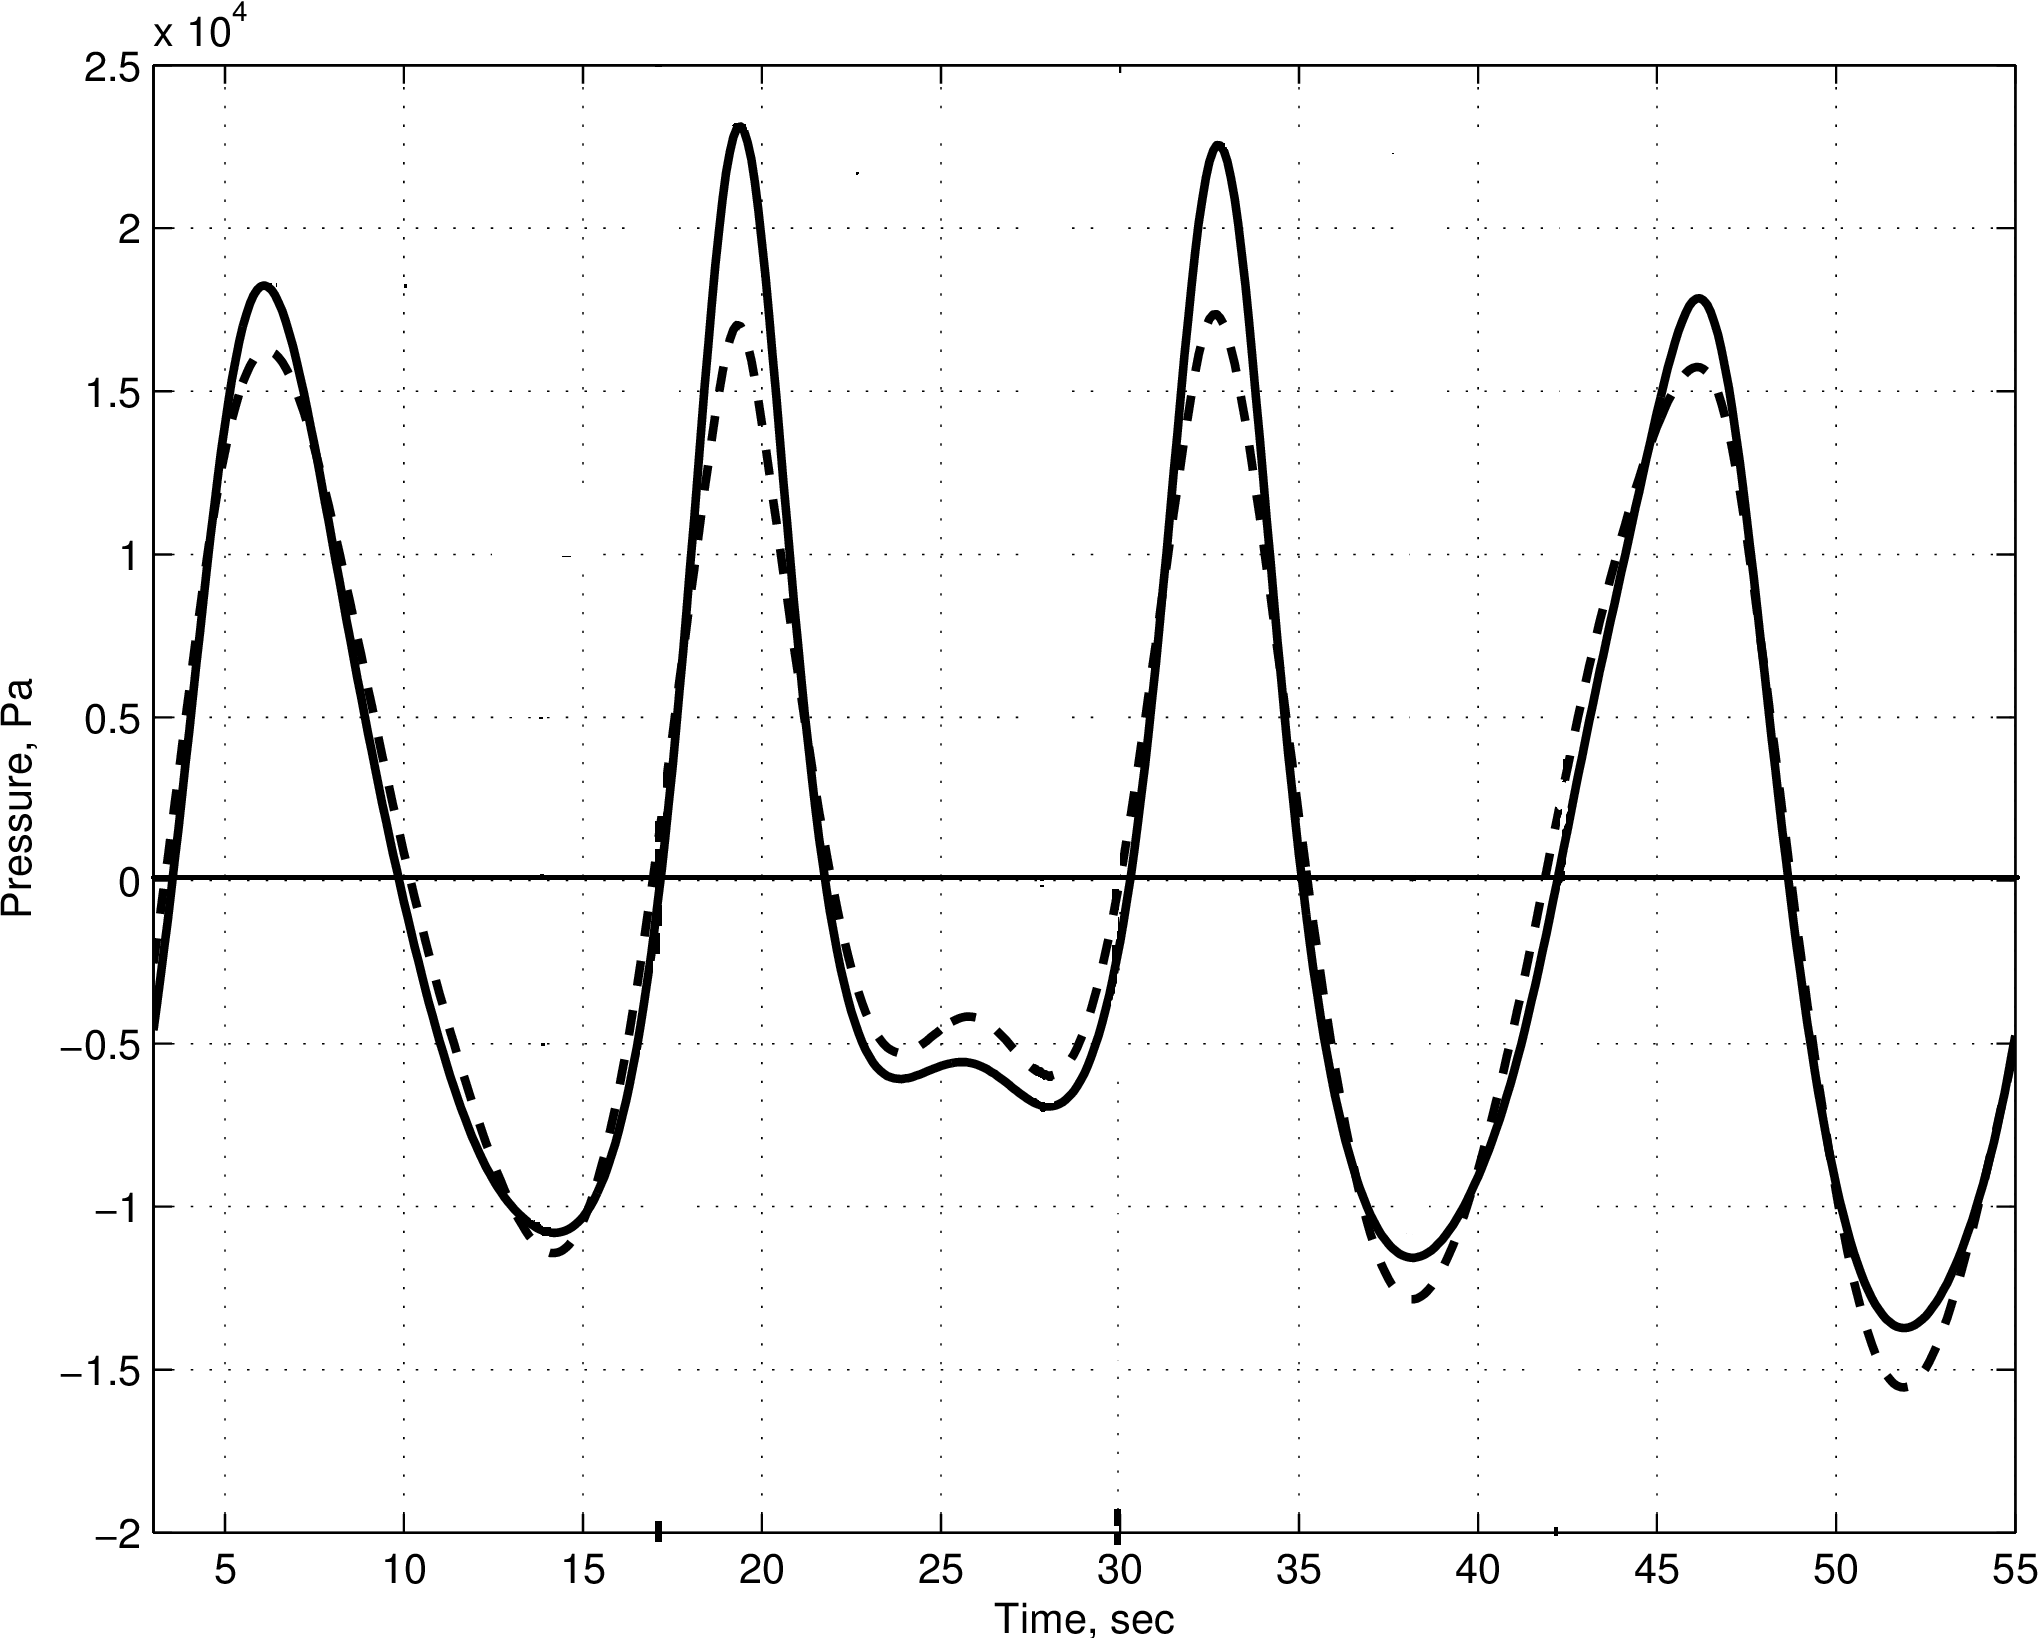
\includegraphics [width=0.7\linewidth] {compareNonlinTheory.png}
  \caption{График колебаний придонного давления, рассчитанного по нелинейной теории (сплошная линия)и по линейной теории (пунктирная линия) для начальной волны c амплитудой A=1.9 м и крутизной k=0.08 }
  \label{img:compareNonlinTheory}
\end{figure}
\FloatBarrier
При этом, как видно из рис.\ref{img:compareNonlinTheory}, недооценка максимумов давления примерно в 2 раза меньше чем переоценка минимумов. Таким образом при решении прямой задачи и нахождения смещения поверхности по данным датчика придонного давления, линейная теория будет недооценивать высоту гребня волны и переоценивать впадину, при этом недооценка высоты как минимум в 2 раза больше переоценки. Т.е. во время регистрации датчиком сильнонелинейных процессов, например таких как волна-убийца, высота, регистрируемых волн будет недооценена.
\begin{figure} [h]
  \center
  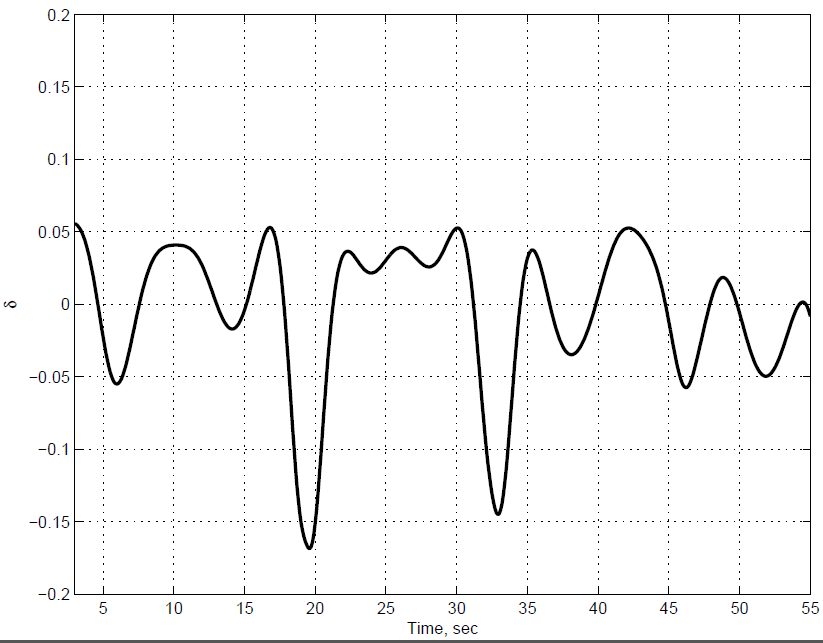
\includegraphics [width=0.7\linewidth] {relErrorNonlin.png}
  \caption{Относительное отклонение $\delta(t)$ придонного давления рассчитанного по линейной и нелинейной формулам для начальной волны с амплитудой A=1.9м и крутизной k=0.08}
  \label{img:relErrorNonlin}
\end{figure}
\FloatBarrier

Рис.\ref{img:compareNonlinTheory} и рис.\ref{img:relErrorNonlin} показывает, что при применении линейной и нелинейной теории к анализу сильнонелинейных процессов отличия по величине могут достигать 17\%. При этом линейная теория существенно сильнее недооценивает уровень жидкости или придонное давление, чем переоценивает его.

Для оценки влияния нелинейности на ошибку в определении линейной теорией уровня жидкости  или давления на дне представим график зависимости среднего значения параметра $\delta(t)*100$ от крутизны начальной волны.
\begin{figure} [h]
  \center
  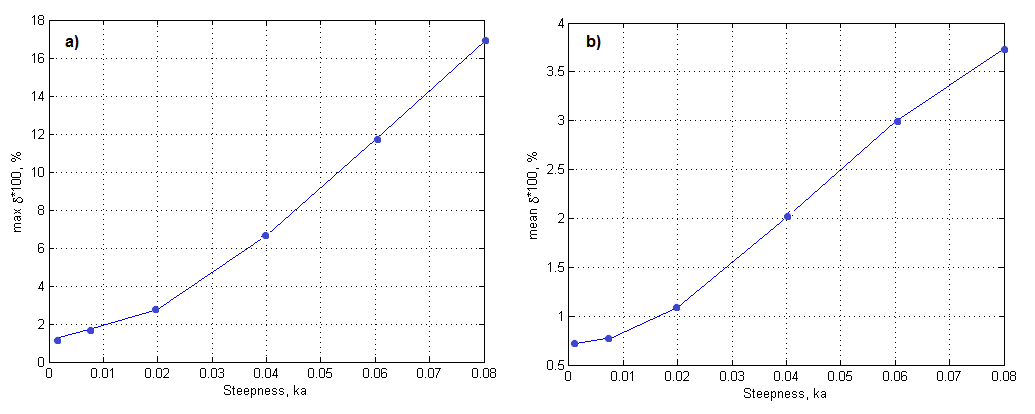
\includegraphics [width=170 mm] {deltaPress.png}
  \caption{Зависимость a)максимума и b) среднего коэффициентов $\delta(t)*100$ от крутизны начальной волны ka, рассчитанного по линейной и нелинейной формулам}
  \label{img:deltaPress}
\end{figure}
\FloatBarrier
Как показано на рис.\ref{img:deltaPress},  при минимальном значении параметра крутизны ka равном 0.0012 среднее значение относительного отклонения составляет менее 1\%, при максимальном ka=0.08 около 4\%. Таким образом можно сделать вывод, что в среднем при сильной нелинейности регистрируемого процесса недооценка величины придонного давления будет составлять около 4\%. В отдельных же случаях, как это следует из рис.\ref{img:deltaPress} может достигать 17\%. Можно предположить что обе зависимости будут хорошо аппроксимироваться функцией $th(ka)$.

%Больше писать по графику относительного отклонения в каких случаях именно

Оценки ошибок линейной теории при регистрации сильнонелинейных процессов приведенные выше справедливы только для величины придонного давления или уровня жидкости.  Проведем оценку размаха колебаний придонных давлений рассчитанных с использованием линейной и нелинейной теории, для этого будем рассматривать сигнал пульсаций давлений как набор индивидуальных волн, которые будут обладать своей высотой(или размахом) и периодом.

\begin{figure} [h]
  \center
  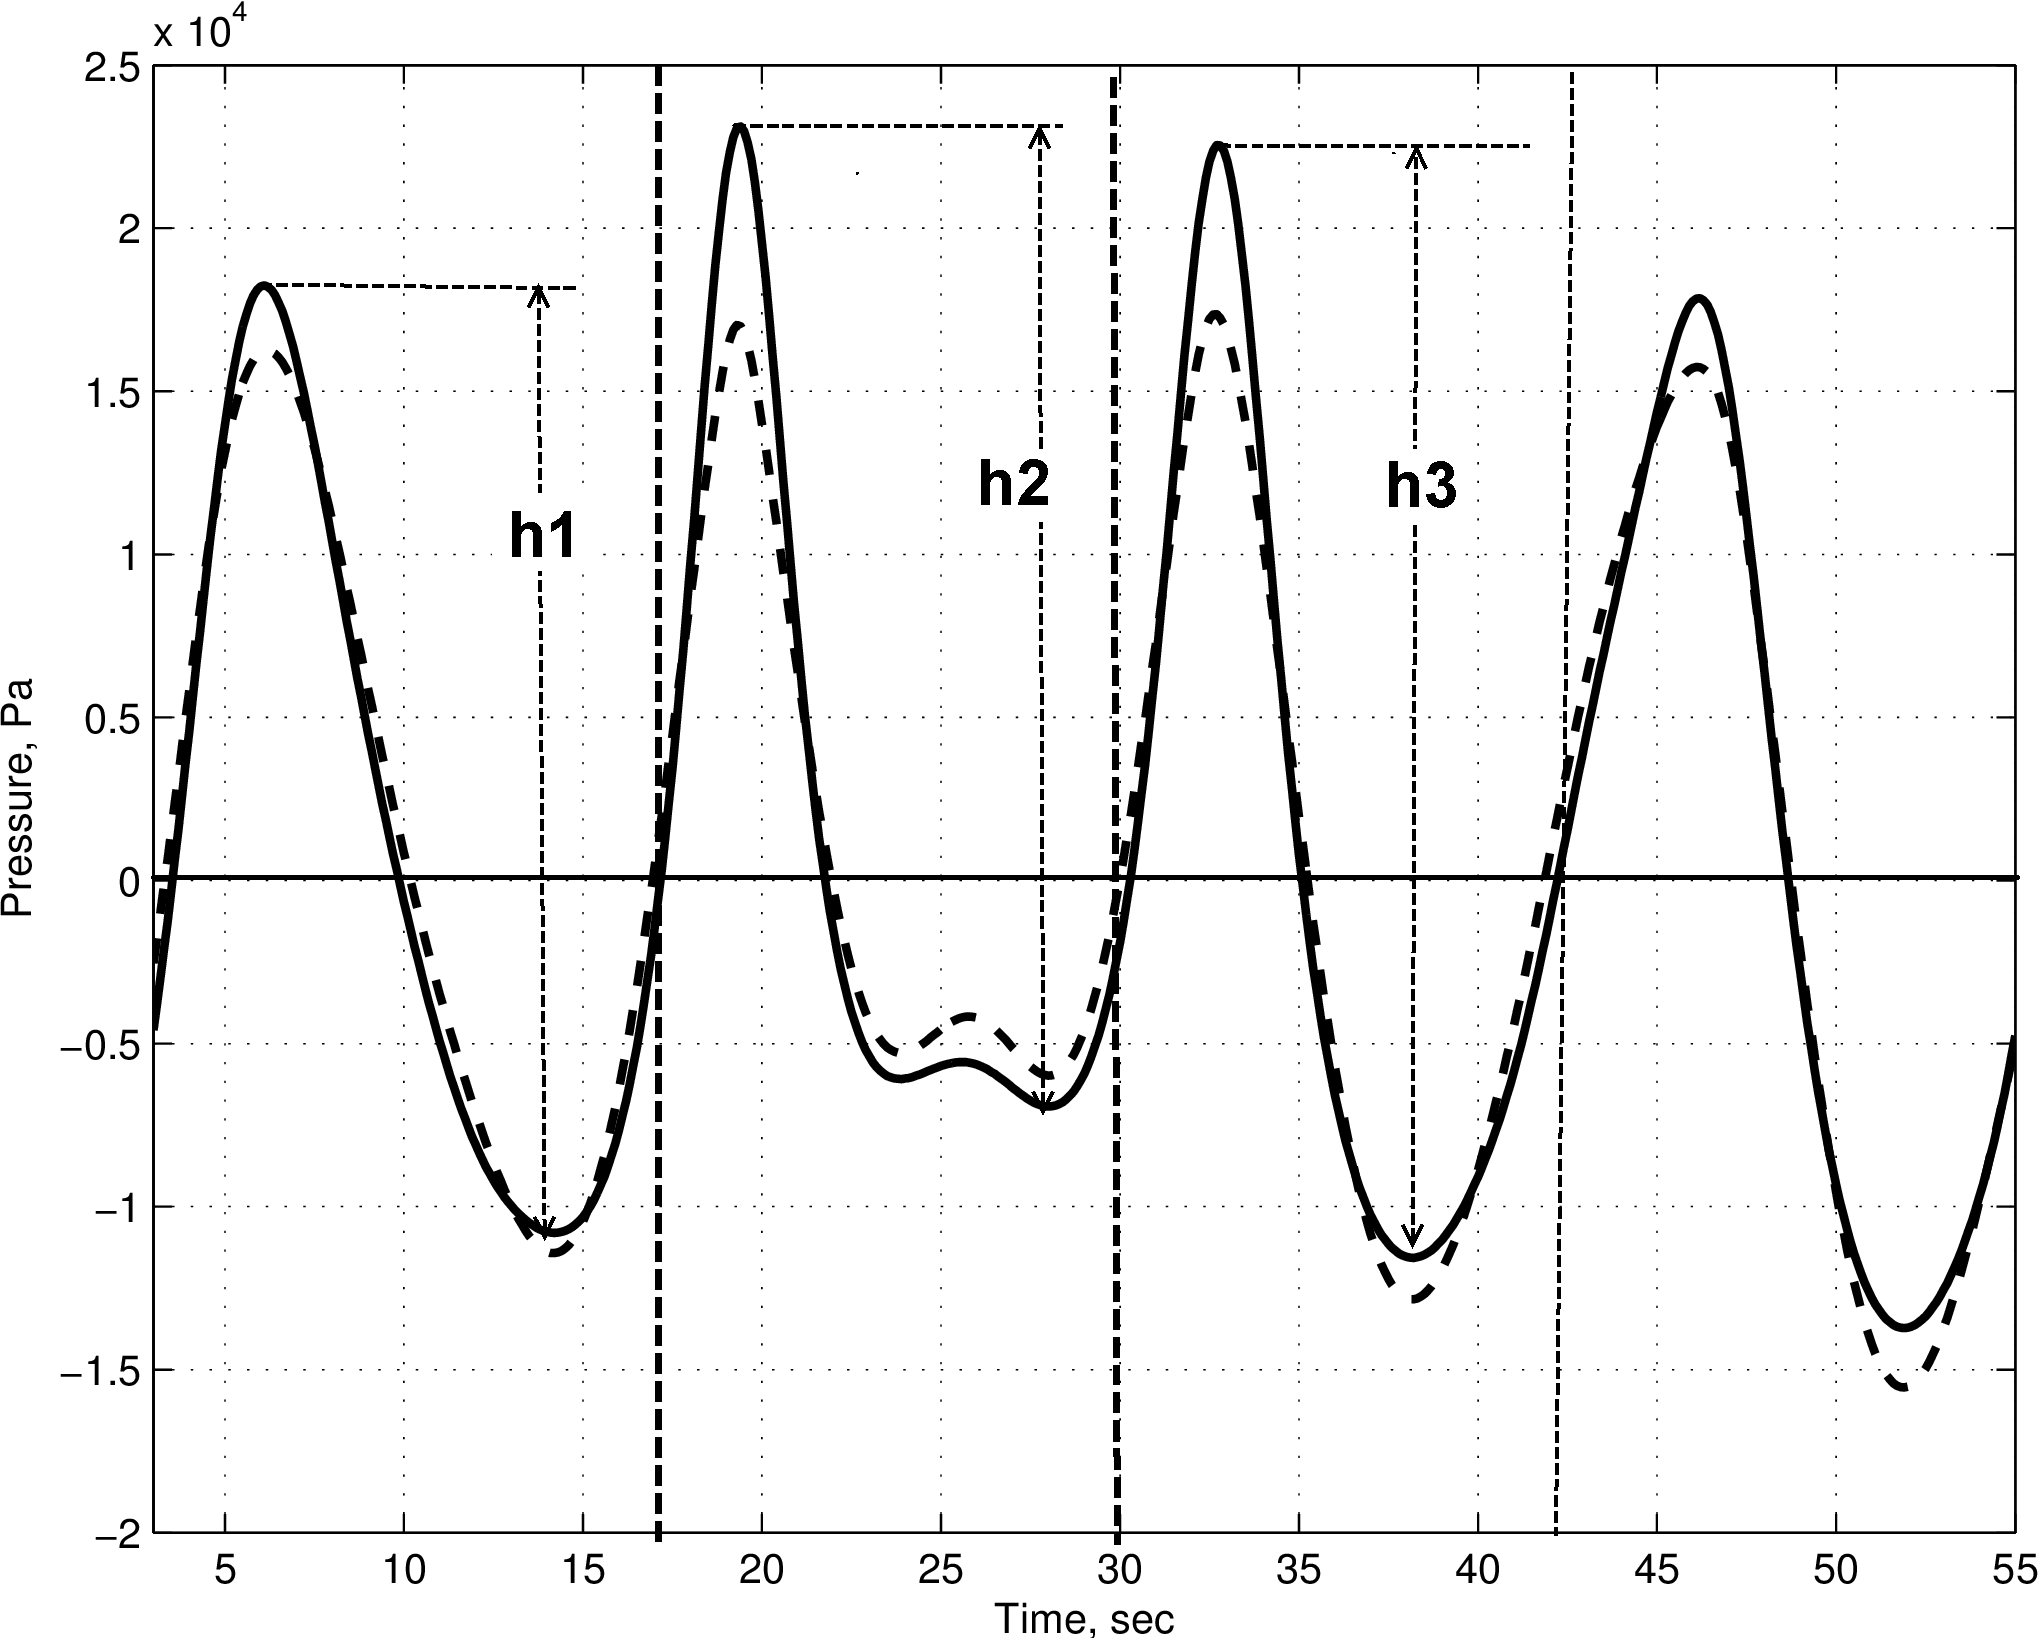
\includegraphics [width=0.7\linewidth] {schemeNonlin.png}
  \caption{Схематичное представление размаха колебаний давления.}
  \label{img:schemeNonlin}
\end{figure}
\FloatBarrier

На рис.\ref{img:schemeNonlin} представлено схематичное изображение данного представления, на этом рисунке h1, h2, h3 - величины размаха индивидуальных колебания давления на дне. В дальнейшем будем называть такие колебания «волнами давления», применяя к ним сложившуюся для поверхностных волн терминологию.

Следуя этой методике были вычислены величины размаха колебания придонных давлений.
\begin{figure} [h]
  \center
  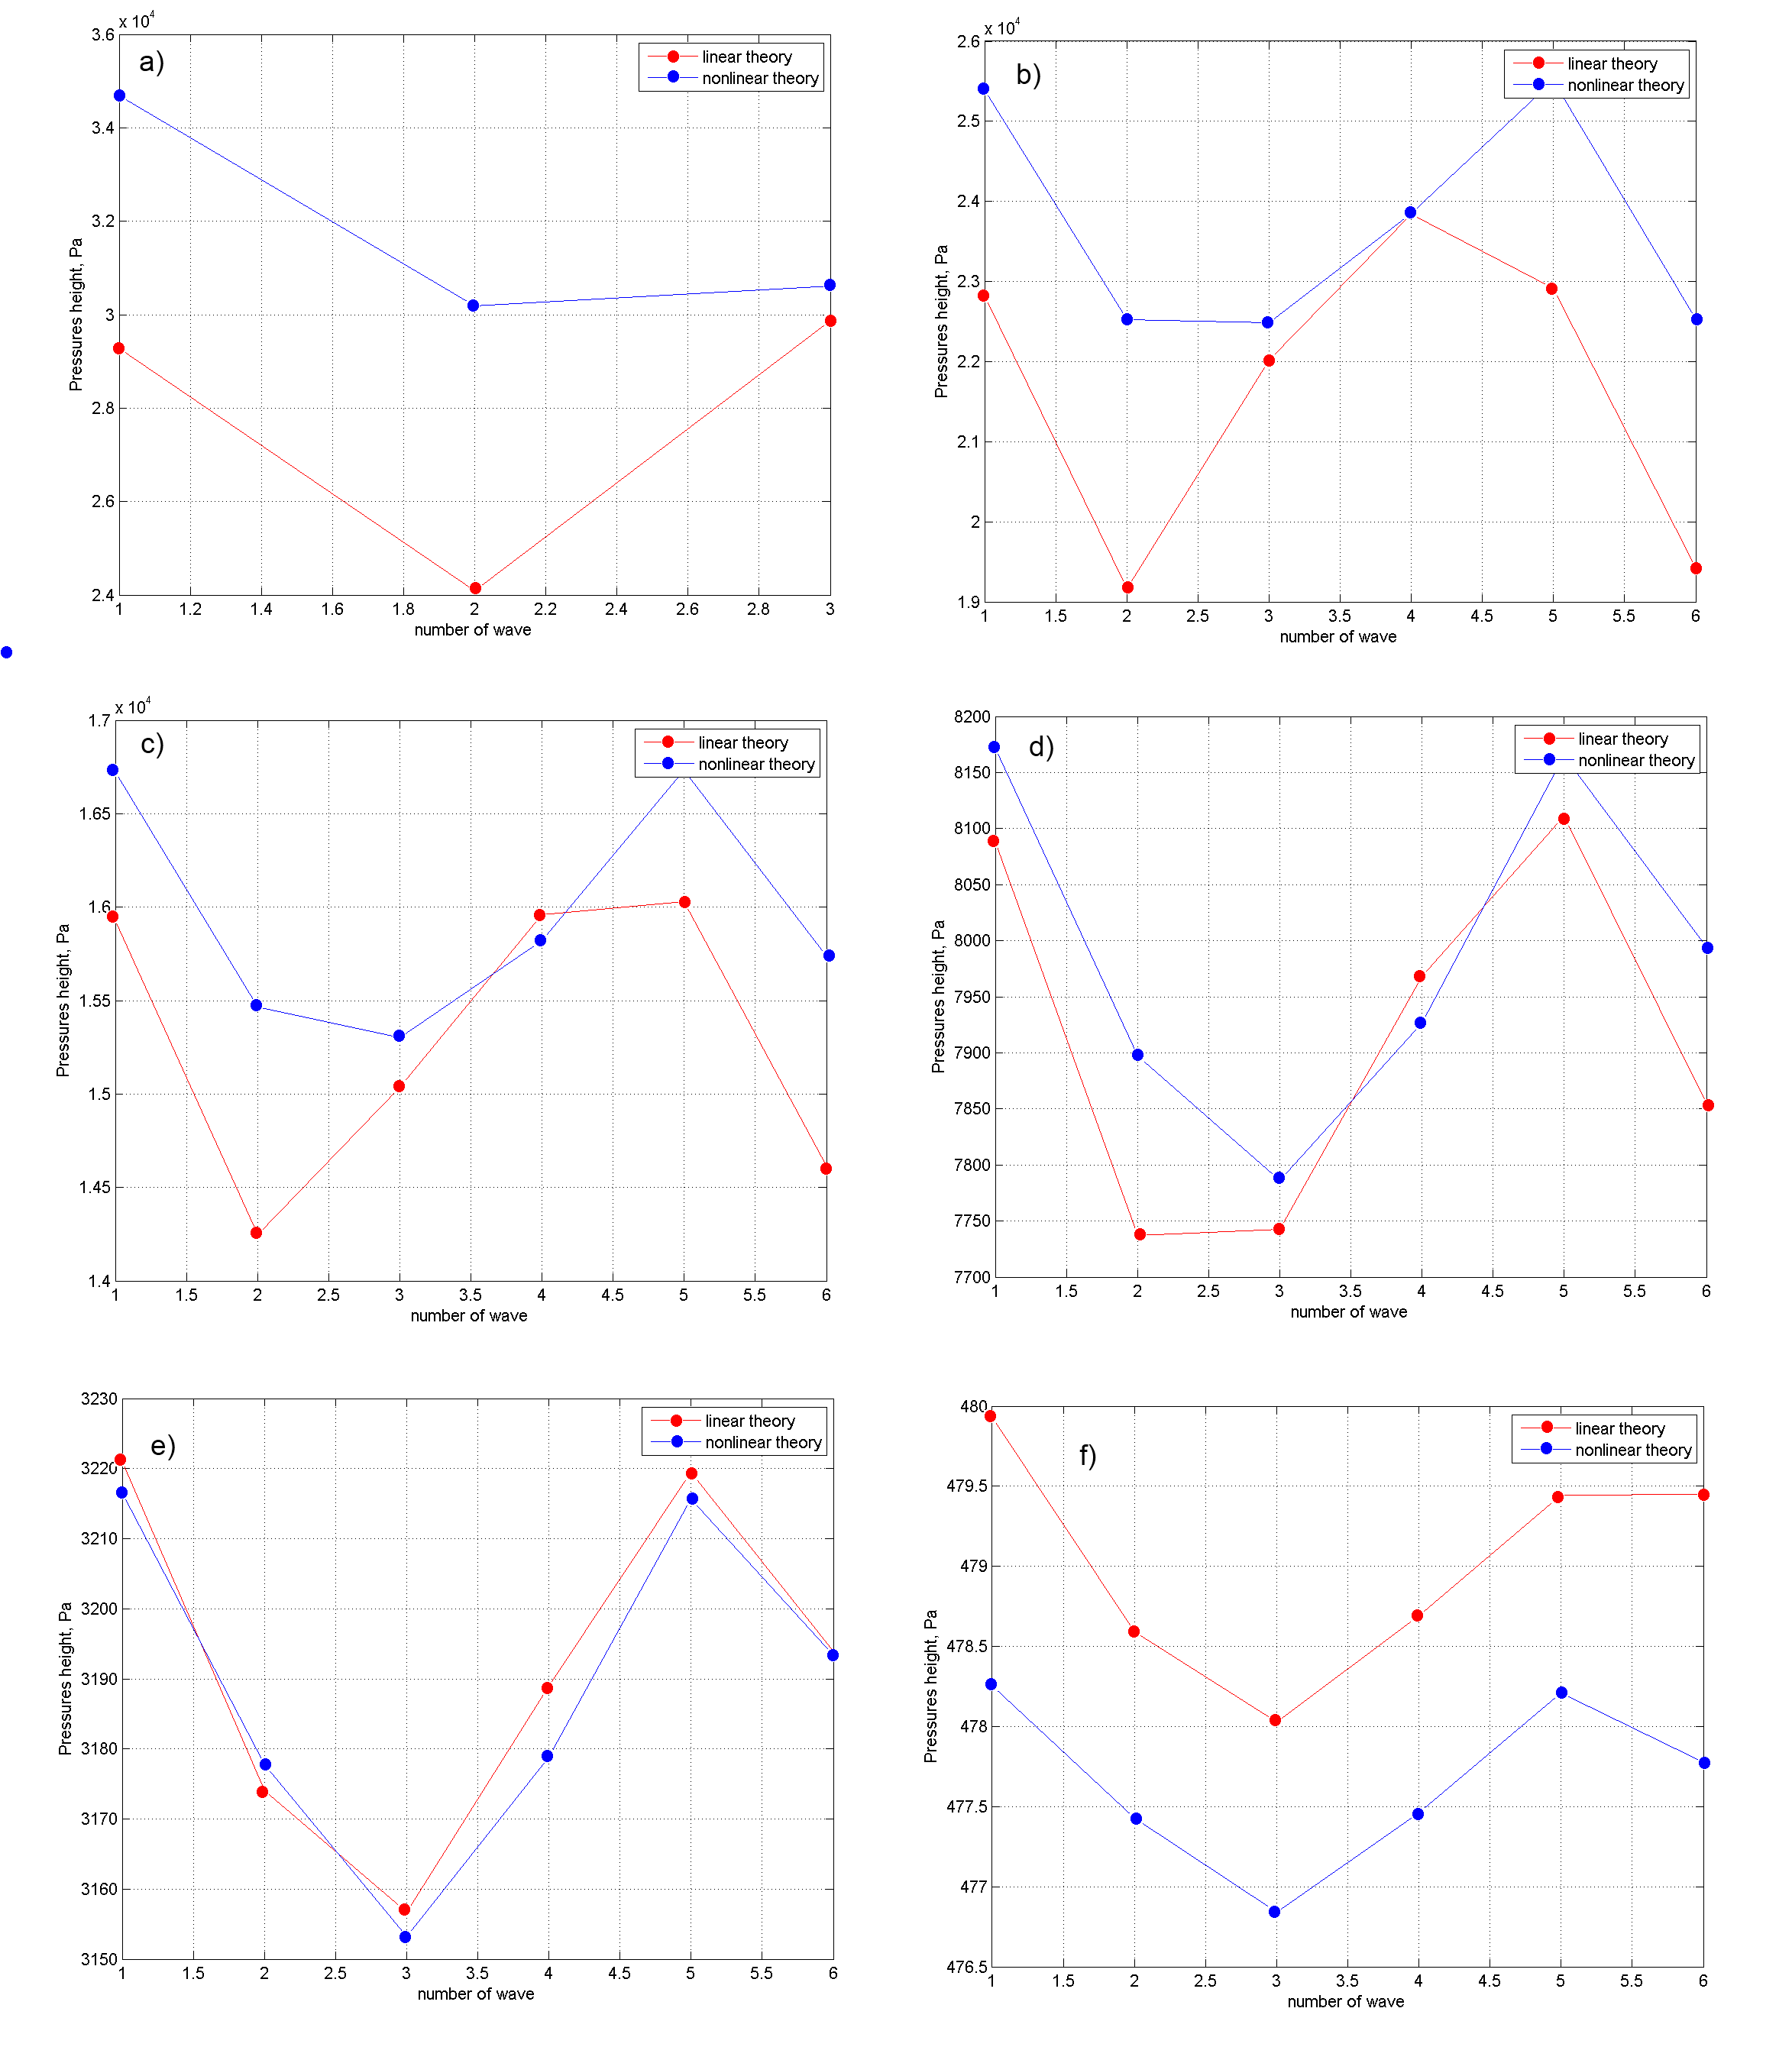
\includegraphics [width=1\linewidth] {compareDeltaH.png}
  \caption{Сравнение размахов колебания придонных давлений, полученных по линейной (красные точки) и нелинейной(синие точки) формулам, при различных крутизнах начальных волн: a) ka=0.08 b) ka=0.06 c) ka=0.04 d) ka=0.02 e) ka=0.008 f) ka=0.0012 }
  \label{img:compareDeltaH}
\end{figure}
\FloatBarrier
На рис.\ref{img:compareDeltaH} представлено сравнение размаха колебаний давлений для случаев с различной крутизной начальной волны. Из этого рисунка можно сделать вывод, что при решении обратной задачи (т.е. нахождения смещения водной поверхности по данным датчика придонного давления) линейная теория в условиях сильнонелинейного процесса, может сильно недооценивать не только уровень жидкости, но и высоту волнения.

%обсмаковать график больше

При уменьшении нелинейности процесса линейная теория приближается к истинному придонному давлению и в конечном счете начинает немного переоценивать высоты волн. На рис.\ref{img:compareDeltaH}f особенно хорошо видно, что отличие линейной теории от нелинейной составляет примерно такую же величину как и отличия высот индивидуальных   волн давления, в то время как величина отличий колебаний индивидуальных высот волн давления прямо говорит о степени нелинейности.  Т.е. чем больше нелинейность, тем больше отличие в показаниях.

Для анализа относительного отклонения подходов размахов колебания давлений, основанных на формулах (\ref{eq:pressNonlin})  и (\ref{eq:pressLin}), введем коэффициент подобный (\ref{eq:relatError}).
\begin{equation}\label{eq:relatErrorH}
\delta_H(i)=\frac{H_{nonlin}(i)-H_{lin}(i)}{H_{max}}
\end{equation}

где  i – номер индивидуального колебания или «волны давления»,  $H_{nonlin}(i)$ - размах колебаний придонного давления, рассчитанный по нелинейной формуле (\ref{eq:pressNonlin}) для i-ой волны; $H_{lin}(i)$  - размах колебаний придонного давления, рассчитанный по формуле линейной теории (\ref{eq:pressLin}) для той же волны; $H_{max}$ - максимальное значение величины размахов колебаний, рассчитанные по нелинейной формуле.

\begin{figure} [h]
  \center
  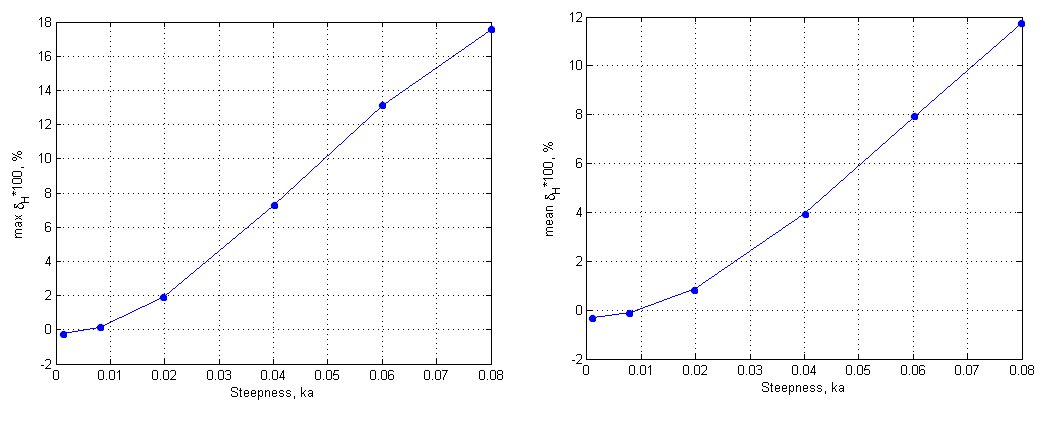
\includegraphics [width=170 mm] {deltaH.png}
  \caption{Зависимость a)максимума и b)среднего коэффициентов $\delta_H(i)*100$  от крутизны начальной волны $ka$, рассчитанного по формулам линейной и нелинейной теории}
  \label{img:deltaH}
\end{figure}
\FloatBarrier

На рис.\ref{img:deltaH} представлена зависимость максимума и среднего коэффициентов $\delta_H(i)$  от крутизны начальной волны $ka$. Из рис.\ref{img:deltaH}b Можно сделать вывод что в среднем недооценка колебания линейной теорией размахов колебания придонного давления колеблется от 12\% до -0.2\%. Отрицательное значение параметра   говорит о переоценке линейной теорией истинного размаха колебаний давления на дне. При этом недооценка линейной теорией размахов колебаний давления во время сильнонелинейных процессов может достигать 18\%. Переоценка же относительно линейных процессов составляет не менее 0.02\%.

Так же стоит отметить, что при решении задачи о нахождении смещения поверхности по данным датчика придонного давления, анализ сильнонелинейных процессов необходимо проводить очень осторожно и учитывать, что линейная теория значительно занижает высоты поверхностных волн, развивающихся в сильнонелинейных процессах, это занижение может достигать 18\%.

\section{Исследование влияния нелинейных эффектов на связь поверхностных волн и придонного давления с использованием слабодисперсионной модели}

\subsection{Связь колебаний водной поверхности с вариациями давления}

В измерениях с использованием донных регистраторов давления из формулы \eqref{GrindEQ__9_} легко вычислить колебания эффективного смещения \textit{$\xi$(x,y,t)}. Она совпадает с реальными колебаниями морской поверхности только при условии пренебрежения негидростатических добавок в \eqref{GrindEQ__8_}, что справедливо только для очень длинных волн. В общем же случае возникает задача нахождения неизвестной функции \textit{$\eta$(x,y,t)} по известной функции $\xi$(x,y,t). Наш подход использует то обстоятельство, что при выводе слабодисперсионной модели нелинейных волн на воде использовалась малость дисперсии, то есть функционала \textit{D}, что автоматически ведет к малости \textit{R} и \textit{Q}. Это означает, что негидростатические поправки к давлению в \eqref{GrindEQ__7_} и \eqref{GrindEQ__8_} должны быть малы. Но тогда в малых слагаемых возможно отождествление функций \textit{$\eta$(x,y,t)} и $\xi$(x,y,t). В результате формула \eqref{GrindEQ__8_} может быть обращена

\begin{equation} \label{GrindEQ__10_}
\eta \approx \xi +\frac{1}{2g} \left[h^{2} +2h\xi +\xi ^{2} \right]R+\frac{1}{g} (h+\xi )Q.
\end{equation}


Такое же приближение необходимо сделать в функциях \textit{R} и \textit{Q}. Но обе функции зависят от поля скоростей, а не поля смещения -- смотри \eqref{GrindEQ__4_} и \eqref{GrindEQ__5_}. Таким образом, задача свелась к вычислению поля скоростей по заданному полю эффективного смещения, и для этого возможно использование уравнения \eqref{GrindEQ__1_} или \eqref{GrindEQ__2_}, которые с нужной точностью записываются как

\begin{equation} \label{GrindEQ__11_}
\frac{\partial \xi }{\partial t} +{\rm div}\left[\left(h+\xi \right)\vec{u}\right]=0,
\end{equation}

\begin{equation} \label{GrindEQ__12_}
\frac{\partial \vec{u}}{\partial t} +(\vec{u}\nabla )\vec{u}+g\nabla \xi =0.
\end{equation}


В общем случае волнового поля в бассейне переменной глубины поле скоростей может быть определено только численно по полю смещения, что означает невозможность получения аналитических зависимостей для искомой задачи. На практике, однако, волнение на море представляет собой две системы волн: ветровые и зыбь, каждая из которых имеет узкую диаграмму направленности. Если зыби нет, то имеем дело с однонаправленными волнами, и для них возможно использовать одномерную систему \eqref{GrindEQ__11_} - \eqref{GrindEQ__12_}. В частности, уравнение \eqref{GrindEQ__11_} трансформируется в


\begin{equation} \label{GrindEQ__13_}
\frac{\partial \xi }{\partial t} +\frac{\partial }{\partial x} \left[\left(h+\xi \right)u\right]=0.
\end{equation}


В случае распространения прогрессивной волны в бассейне постоянной глубины решение уравнения \eqref{GrindEQ__13_} находится в явном виде

\begin{equation} \label{GrindEQ__14_}
u=V\frac{\xi }{h+\xi } ,
\end{equation}


где V -- скорость распространения волны. В результате, мы имеем замкнутую формулу для вычисления смещения водной поверхности

\begin{equation} \label{GrindEQ__15_}
\eta \approx \xi +\frac{1}{2g} \left[h^{2} +2h\xi +\xi ^{2} \right]R.
\end{equation}


где $R$ вычисляется из \eqref{GrindEQ__4_}

\begin{equation} \label{GrindEQ__16_}
R=\frac{\partial ^{2} u}{\partial t\partial x} +u\frac{\partial ^{2} u}{\partial x^{2} } -\left(\frac{\partial {\rm u}}{\partial {\rm x}} \right)^{2} ,
\end{equation}


и скорость \textit{u} - с помощью \eqref{GrindEQ__14_}. Наконец, надо учесть то обстоятельство, что давление измеряется в точке, поэтому все пространственные переменные должны быть заменены на временные с использованием связи

\begin{equation} \label{GrindEQ__17_}
\frac{\partial u}{\partial x} =-\frac{1}{V} \frac{\partial u}{\partial t} .
\end{equation}


В результате, функция \textit{R} записывается в виде

\begin{equation} \label{GrindEQ__18_}
R=-\frac{1}{V} \left(1-\frac{u}{V} \right)\frac{\partial ^{2} u}{\partial t^{2} } -\frac{1}{V^{2} } \left(\frac{\partial {\rm u}}{\partial t} \right)^{2} ,
\end{equation}


Важно отметить, что для вычисления смещения водной поверхности в точке, мы должны знать вариации давления в точке и согласно \eqref{GrindEQ__18_} - скорость распространения волны \textit{V}. На самом же деле, в \eqref{GrindEQ__18_} всюду входит скорость течения и скорость волны не независимо, а через комбинацию u/V. Последняя же находится из \eqref{GrindEQ__14_} как


\begin{equation} \label{GrindEQ__19_}
\frac{u}{V} =\frac{\xi }{h+\xi } ,
\end{equation}


так что знание скорости распространения волны не является обязательным. Таким образом, мы можем привести окончательное выражение вычисления смещения водной поверхности


\begin{equation} \label{GrindEQ__20_}
\eta \approx \xi -\frac{1}{2g} \left[h^{2} +2h\xi +\xi ^{2} \right]\left[\frac{h}{h+\xi } \frac{\partial ^{2} }{\partial t^{2} } \left(\frac{\xi }{h+\xi } \right)+\left\{\frac{\partial }{\partial t} \left(\frac{\xi }{h+\xi } \right)\right\}^{2} \right].
\end{equation}


Формула \eqref{GrindEQ__20_} позволяет оценить смещение водной поверхности по измерениям донного давления. Отметим, что оно должно измеряться достаточно аккуратно, чтобы иметь возможность вычислить ее вторую производную. Формальным ограничением данного подхода является малость дисперсионных эффектов, так что волна должна быть достаточно длинной. При этом на амплитуду ее не накладывается никаких ограничений.

Если к тому же волна имеет достаточно малую амплитуду, то учитывая и малость дисперсии, во всех «негидростатических» членах можно пренебречь влиянием нелинейности. Тогда формула \eqref{GrindEQ__20_} принимает очень простой вид


\begin{equation} \label{GrindEQ__21_}
\eta \approx \xi -\frac{h}{2g} \frac{\partial ^{2} \xi }{\partial t^{2} } .
\end{equation}

\subsection{Примеры расчета поверхностных волн по вариациям донного давления для условий Охотского моря}

Рассмотрим несколько примеров аналитического вычисления смещения водной поверхности, используя модельные записи вариаций давления на дне. При этом мы будем использовать эффективное смещение, чтобы обе характеристики имели одну размерность.

А) Распространение монохроматической волны


\begin{equation} \label{GrindEQ__22_}
\xi (t)=A\sin (\omega t).
\end{equation}


В малоамплитудном приближении смещение водной поверхности остается синусоидальным и синфазным вариациям давления

\begin{equation} \label{GrindEQ__23_}
\eta(t)=A\left(1+\frac{h\omega^{2} }{2g} \right)\sin(\omega t).
\end{equation}


Как видим, амплитуда колебаний свободной поверхности превышает гидростатическое значение.

Для оценки отличия малоамлитудного приближения от гидростатического приближения, построим графики $\eta(t)$ и $\xi(t)$, с параметрами характерными для шельфа Охотского моря, которые были получены во время натурных экспериментов \cite{Kuznetsov_EGU2013}. На шельфе Охотского моря наиболее часто встречаются волны с периодами 4-7 секунд, а наиболее часто наблюдаемые амплитуды волн колеблются в диапазоне от 10 см до 40 см. Натурные наблюдения при этом проводились на глубинах от 5 м до 20 м, с помощью датчиков придонного давления. На рис.\ref{img:graph22_23} приведены функции $\eta(t)$ и $\xi(t)$ для волны с периодом 4 секунды в бассейне глубиной 20 метров. Отклонения от гидростатики довольно слабые. Рис. \ref{img:coeffAttenua} демонстрирует влияние негидростатических эффектов через отношение $\frac{\eta(t)}{\xi(t)}$. Для условий наблюдений в зависимости от глубины и периода волны разница может достигать 5\%. Аналогичные выводы для периодических волн сделаны в \cite{Oliveras_2012} для периодических волн в лотке.

\begin{figure} [ht]
  \center
  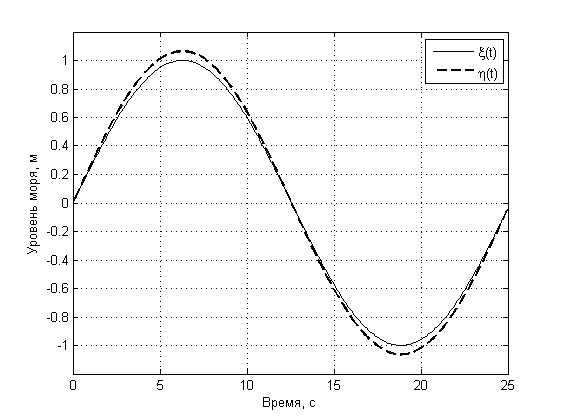
\includegraphics [width=0.5\linewidth] {graph22_23_A1W4h20.png}
  \caption{Смещение водной поверхности, рассчитанное по малоамплитудному приближению (пунктирная линия) и гидростатическому приближению (тонкая линия) для волны с амплитудой A=1м и периодом 4 секунд и глубиной бассейна 20 метров.}
  \label{img:graph22_23}
\end{figure}
\FloatBarrier

\begin{figure} [ht]
  \center
  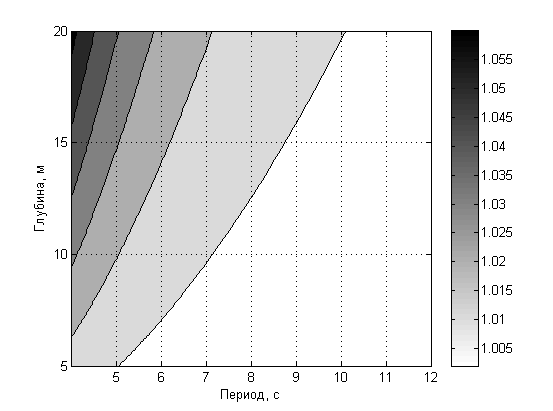
\includegraphics [width=0.5\linewidth] {coeffAttenua.png}
  \caption{Отношение $\frac{\eta (t)}{\xi (t)} $в зависимости от периода волн, наиболее часто наблюдаемых на шельфе Охотского моря и глубины. }
  \label{img:coeffAttenua}
\end{figure}
\FloatBarrier




Б) Распространение гауссового импульса

\begin{equation} \label{GrindEQ__24_}
\xi (t)=A\exp \left(-\frac{4t^{2} }{T^{2} } \right),
\end{equation}


где \textit{T} -- характерная длительность импульса. В этом случае колебания свободной поверхности есть


\begin{equation} \label{GrindEQ__25_}
\eta (t)=A\left[1+\frac{4h}{gT^{2} } -\frac{32t^{2} }{gT^{4} } \right]\exp \left(-\frac{4t^{2} }{T^{2} } \right).
\end{equation}


Форма колебаний давления (через эффективное смещение) и свободной поверхности показаны на рис. \ref{img:graph24_25}. Как видим, разница между гидростатическим и негидростатическим приближением довольно существенна и достигает 20\%. Рис. \ref{img:coeffAttenua25} показывает, что расхождение в показаниях малоамплитудного и гидростатического приближений  для гассового импульса может достигать 50\%  при условиях, характерных для шельфа Охотского моря. Оно существенно больше, чем в случае монохроматической волны.

\begin{figure} [ht]
  \center
  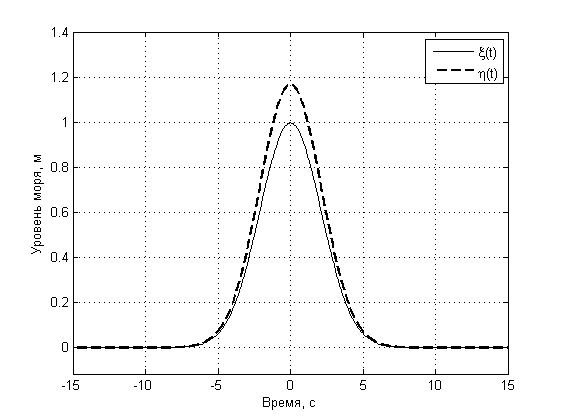
\includegraphics [width=0.5\linewidth] {graph24_25_A1W6h15.png}
  \caption{Смещение водной поверхности, рассчитанное по малоамплитудному приближению (пунктирная линия) и гидростатическому приближению (тонкая линия) для импульса с амплитудой A=1 м, характерной длительностью импульса 6 секунд; глубина бассейна - 15 метров.}
  \label{img:graph24_25}
\end{figure}
\FloatBarrier

\begin{figure} [ht]
  \center
  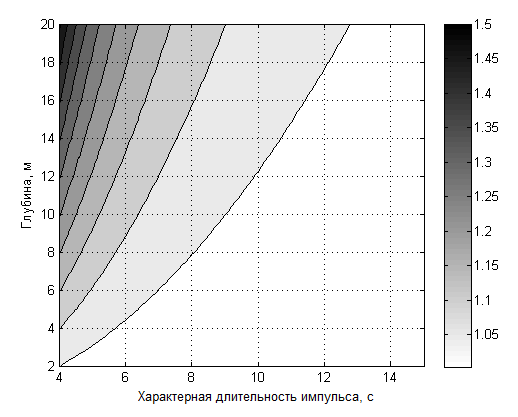
\includegraphics [width=0.5\linewidth] {coeffAttenua25.png}
  \caption{Отношение $\frac{\eta (t)}{\xi (t)} $для гауссового импульса в зависимости от характерной длительности импульса и глубины. }
  \label{img:coeffAttenua25}
\end{figure}
\FloatBarrier

\subsection{Давление на дно, вызванное прохождением уединенной волны в прибрежной зоне}
Воспользуемся здесь одномерным вариантом уравнений Железняка -- Пелиновского для волн в бассейне постоянной глубины \cite{Zhel_Pel_1985}


\begin{equation} \label{GrindEQ__1_}
\frac{\partial \eta }{\partial t} +\frac{\partial }{\partial x} \left[\left(h+\eta \right)u\right]=0,
\end{equation}

\begin{equation} \label{GrindEQ__2_}
\frac{\partial u}{\partial t} +u\frac{\partial u}{\partial x} +g\frac{\partial \eta }{\partial x} =D\left\{\eta ,u\right\},
\end{equation}


 где \textit{$\eta$(x,t)} -- смещение водной поверхности, \textit{u(x,t)} -- усредненная по глубине скорость течения, \textit{h} -- невозмущенная постоянная глубина бассейна, \textit{g} -- ускорение силы тяжести, и \textit{D} -- функционал, определяющий влияние малой дисперсии


\begin{equation} \label{GrindEQ__3_}
D=\frac{1}{3\left(h+\eta \right)} \frac{\partial }{\partial x} \left[\left(h+\eta \right)^{3} R\right],
\end{equation}

\begin{equation} \label{GrindEQ__4_}
R=\frac{\partial ^{2} u}{\partial t\partial x} +u\frac{\partial ^{2} u}{\partial x^{2} } -\left(\frac{\partial u}{\partial x} \right)^{2} .
\end{equation}


 Как отмечается в работе \cite{Fedotova_2008}, форма записи системы \eqref{GrindEQ__1_} -- \eqref{GrindEQ__4_} уравнений может иметь важное значение при конструировании эффективных численных алгоритмов. Так, уравнения Железняка-Пелиновского, как и уравнения Федотовой и Хакимзянова более удобны для численной реализации, поскольку, в отличие от системы Грина-Нагди уравнения \eqref{GrindEQ__1_} -- \eqref{GrindEQ__4_} не содержат вторых производных по времени от искомой функции.

Если нелинейность достаточно мала, то в функционале дисперсии можно оставить только линейные по полю слагаемые


\begin{equation} \label{GrindEQ__5_}
D=\frac{h^{2} }{3} \frac{\partial ^{3} u}{\partial t\partial x^{2} } .
\end{equation}


 В этом случае система \eqref{GrindEQ__1_} -- \eqref{GrindEQ__2_} с дисперсионным слагаемым \eqref{GrindEQ__5_} сводится к системе Перегрина \cite{Peregrinde}. Отметим, что при слабой нелинейности возможно дальнейшее упрощение дисперсионного функционала, который может быть представлен в нескольких эквивалентных формах


\begin{equation} \label{GrindEQ__6_}
D_{1} =\frac{h^{2} }{3} \frac{\partial ^{3} u}{\partial t\partial x^{2} } ,     D_{2} =-\frac{gh^{2} }{3} \frac{\partial ^{3} \eta }{\partial x^{3} } ,     D_{3} =-\frac{h}{3} \frac{\partial ^{3} \eta }{\partial t^{2} \partial x} ,     D_{4} =\frac{h}{3g} \frac{\partial ^{3} u}{\partial t^{3} } .
\end{equation}


Наличие разных форм дисперсионного функционала ведет в линейном приближении к различным формам дисперсионного соотношения, одинаковым в области длинных волн ($kh<<1$), но различным в более коротковолновой области. Эти различия можно использовать при численном моделировании уравнений Буссинеска, обеспечивая лучшую устойчивость численных схем. Так, использование слагаемых $D_2$ и $D_4$ ведет к неустойчивости линейных решений на малых масштабах; см. дискуссию в \cite{pel_2006}.

Здесь мы рассмотрим влияние дисперсии на солитонные решения системы \eqref{GrindEQ__1_} -- \eqref{GrindEQ__2_}. Переходя в систему отсчета, движущую со скоростью солитона \textit{V}, уравнение \eqref{GrindEQ__1_} сразу интегрируется


\begin{equation} \label{GrindEQ__7_}
u=V\frac{\eta }{h+\eta } ,
\end{equation}


 что позволяет исключить скорость течения или смещение водной поверхности. Соответственно уравнение \eqref{GrindEQ__2_} с Перегриновским дисперсионным слагаемым \eqref{GrindEQ__5_} сводится к обыкновенному дифференциальному уравнению второго порядка


\begin{equation} \label{GrindEQ__8_}
g\eta +\frac{u^{2} }{2} -Vu=-\frac{Vh^{2} }{3} \frac{d^{2} u}{dx^{2} } .
\end{equation}


 Удобно здесь исключить смещение водной поверхности с помощью \eqref{GrindEQ__7_} и получить замкнутое уравнение для скорости потока


\begin{equation} \label{GrindEQ__9_}
\frac{ghu}{V-u} +\frac{u^{2} }{2} -Vu=-\frac{Vh^{2} }{3} \frac{d^{2} u}{dx^{2} } .
\end{equation}


 Учитывая, однако, линейность дисперсионного слагаемого, мы ограничимся квадратичными нелинейными членами в \eqref{GrindEQ__9_} и учтем, что скорость распространения солитона близка к линейной скорости распространения длинных волн


\begin{equation} \label{GrindEQ__10_}
c=\sqrt{gh} ,
\end{equation}


 что позволяет заменить $V$ на $c$ в малых слагаемых. В результате уравнение \eqref{GrindEQ__9_} упрощается


\begin{equation} \label{GrindEQ__11_}
\frac{h^{2} }{3} \frac{d^{2} u}{dx^{2} } =\left(1-\frac{c^{2} }{V^{2} } \right)u-\left(\frac{1}{2} +\frac{c^{2} }{V^{2} } \right)\frac{u^{2} }{V} .
\end{equation}


 Это уравнение легко решается и определяет периодические (кноидальные) и уединенные волны. В частности, солитонное решение есть


\begin{equation} \label{GrindEQ__12_}
u=U{\rm sech}^{2} \left[Q(x-Vt)\right],
\end{equation}


 где «обратная» ширина солитона и его скорость равны


\begin{equation} \label{GrindEQ__13_}
Q=\sqrt{\frac{3}{4h^{2} } \frac{U/V}{1+\frac{2U}{3V} } } ,        V=c\sqrt{\frac{1+\frac{2U}{3V} }{1-\frac{U}{3V} } } .
\end{equation}


 Мы специально пока не упрощаем подкорневые выражения в \eqref{GrindEQ__13_}, поскольку они включают амплитуду волны скорости, а не смещения. Волна смещения получается из \eqref{GrindEQ__7_} в первом приближении как


\begin{equation} \label{GrindEQ__14_}
\eta =A{\rm sech}^{2} \left[Q(x-Vt)\right],               A=hU/V.
\end{equation}


 В результате мы можем написать окончательные выражения для параметров солитона


\begin{equation} \label{GrindEQ__15_}
Q=\sqrt{\frac{3}{4h^{3} } \frac{A}{1+\frac{2A}{3h} } } ,        V=c\sqrt{\frac{1+\frac{2A}{3h} }{1-\frac{A}{3h} } } .
\end{equation}


 В приближении слабой нелинейности (как в модели Кортевега -- де Вриза) получаются совпадающие результаты \cite{pel_2006, Hammak_1974}


\begin{equation} \label{GrindEQ__16_}
Q_{kdv} =\sqrt{\frac{3A}{4h^{3} } } ,        V_{kdv} =c\left(1+\frac{A}{2h} \right).
\end{equation}


Отличие в свойствах солитона, получаемое в рамках Буссинесковской системы и уравнения Кортевега -- де Вриза, показано на рис.\ref{img:solitonPress_1}. Как видно, практически до предельной амплитуды солитона на мелкой воды ($A/h\sim0.8$) отличия в параметрах не превышает 20\%. Поэтому для грубых расчетов можно использовать более простое уравнение Кортевега -- де Вриза. Аналогичный вывод делался для солитона в жидкости переменной глубины \cite{pel_tal_2010}.

\begin{figure} [h]
  \center
  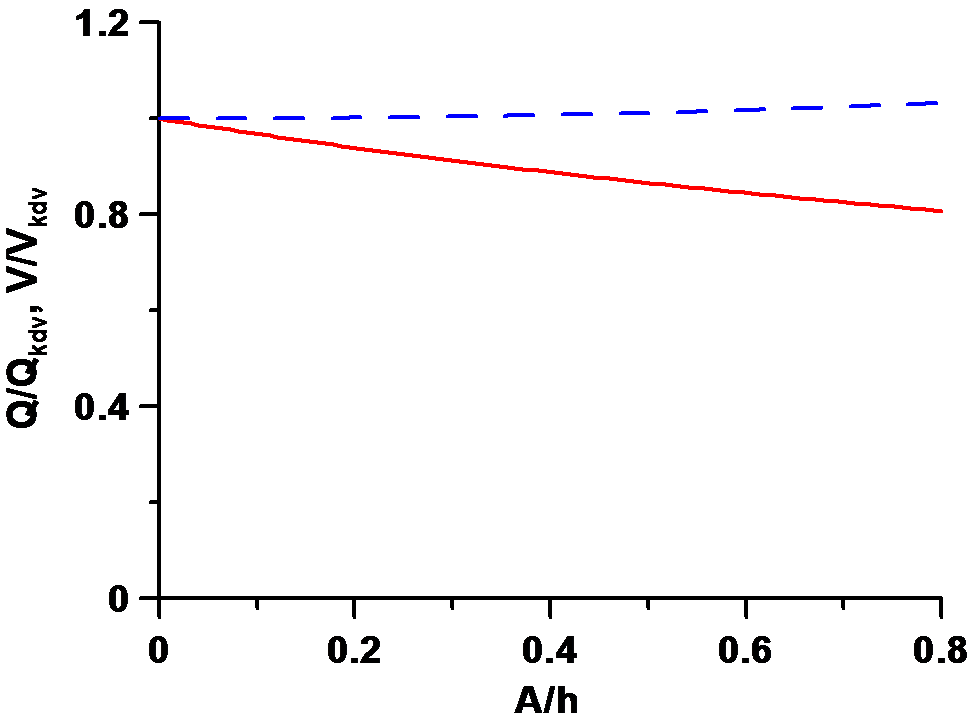
\includegraphics [width=0.7\linewidth] {solitonPress_1.png}
  \caption{Сопоставление параметров солитона в рамках системы Буссинеска и уравнения Кортевега-де Вриза (Q -- сплошная красная линия и V -- штриховая синяя линия)}
  \label{img:solitonPress_1}
\end{figure}
\FloatBarrier






\subsubsection{Давление на дно}

При выводе уравнений Буссинеска удается также получить явное выражение для вертикального профиля давления \cite{Zhel_1985, Zhel_Pel_1985}.


\begin{equation} \label{GrindEQ__17_}
p=p_{atm} +\rho g(\eta -z)+\frac{\rho }{2} \left[z^{2} +2h(z-\eta )-\eta ^{2} \right]R,
\end{equation}


 где $\rho$ - плотность воды, вертикальная координата $z$ направлена вверх и функция \textit{R} определена выражением \eqref{GrindEQ__4_}. Первые два члена в \eqref{GrindEQ__17_} определяют гидростатическое давление, а последние слагаемое -- малую дисперсионную поправку.

Итак, в бассейне постоянной глубины давление на любой глубине выражается через уровень воды и горизонтальную скорость течения. Вертикальное распределение давления показано на рис.\ref{img:solitonPress_2}. Если гидростатическое давление всегда линейно растет с глубиной, то негидростатическая имеет параболический профиль и возрастает с глубиной, если $R<0$ и убывает, если $R>0$ (именно этот случай и показан на рис.\ref{img:solitonPress_2}.

\begin{figure} [h]
  \center
  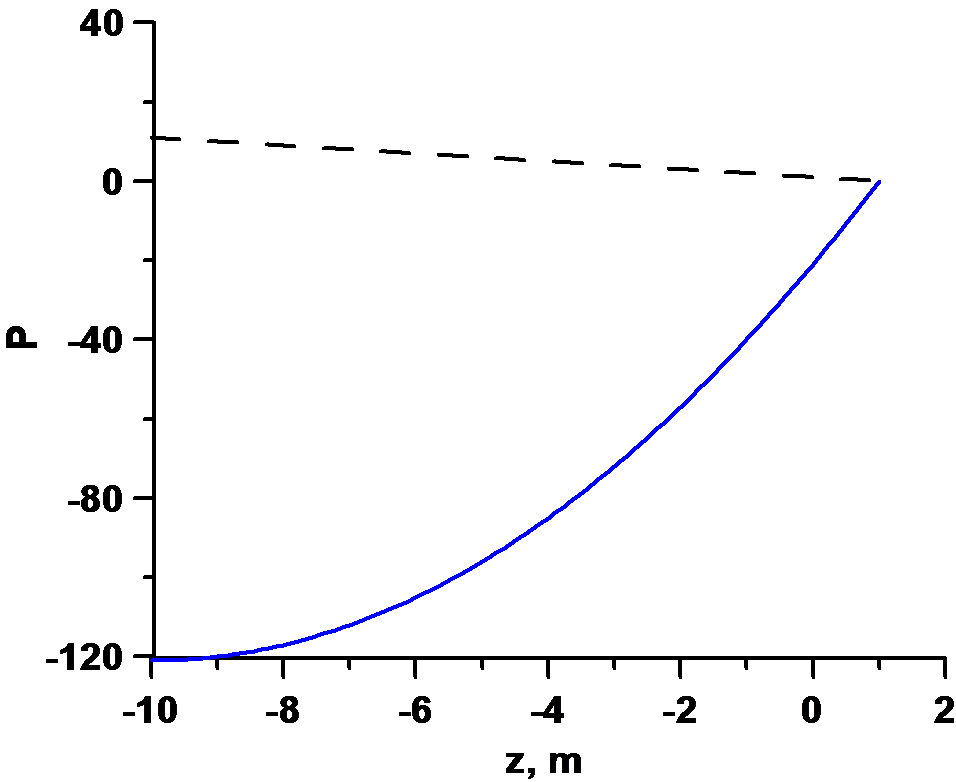
\includegraphics [width=0.7\linewidth] {solitonPress_2.png}
  \caption{Вертикальное распределение давления с глубиной (гидростатическая поправка -- штриховая черная линия, и негидростатическая -- сплошная синяя линия). h = 10 м, $\eta$ = 1 м}
  \label{img:solitonPress_2}
\end{figure}
\FloatBarrier



Давление на дно, вызванное прохождением длинной волны, при условии, что ее амплитуда меньше глубины бассейна, находится из \eqref{GrindEQ__17_}


\begin{equation} \label{GrindEQ__18_}
p\approx p_{atm} +\rho gh+\rho g\eta -\frac{\rho h^{2} }{2} R.
\end{equation}


 Учитывая в $R$ только линейный член по нелинейности, формула \eqref{GrindEQ__18_} преобразуется к виду


\begin{equation} \label{GrindEQ__19_}
p\approx p_{atm} +\rho gh+\rho g\eta -\frac{\rho h^{2} }{2} R,
\end{equation}


 или


\begin{equation} \label{GrindEQ__20_}
p\approx p_{atm} +\rho gh+\rho g\eta _{ef} ,
\end{equation}


 где


\begin{equation} \label{GrindEQ__21_}
\eta _{ef} =\eta +\frac{h^{2} }{2} \frac{\partial ^{2} \eta }{\partial x^{2} } .
\end{equation}


 Последняя формула позволяет понять соотношение между гидростатической (первый член) и негидростатической (второй член) компонентами в флуктуации давления на дне. Эта формула справедлива как для кноидальных, так и уединенных волн на мелкой воде. В частности, для уединенной волны (солитона) получаем


\begin{equation} \label{GrindEQ__22_}
\eta _{ef} =A\left(1+\frac{3A}{2h} \right){\rm sech}^{2} \left[\sqrt{\frac{3A}{4h} } \frac{x-Vt}{h} \right]-\frac{9}{4} \frac{A^{2} }{h} {\rm sech}^{4} \left[\sqrt{\frac{3A}{4h} } \frac{x-Vt}{h} \right].
\end{equation}


 В максимуме поля эффективное смещение равно


\begin{equation} \label{GrindEQ__23_}
\max (\eta _{ef} )=A\left(1-\frac{3A}{4h} \right).
\end{equation}


Отсюда следует, что дисперсионная поправка уменьшает давление на дно, Объяснением этого является тот факт, что более высокочастотные компоненты в спектре волны затухают с глубиной быстрее низкочастотных, что и приводит к ослаблению давления на дно. Более интересным является пространственное распределение давления, показанное на рис.\ref{img:solitonPress_3}. Если для солитонов малой амплитуды профиль давления практически повторяет профиль уединенной волны, то начиная с солитонов с относительной высотой $A/h\sim0.5$, профиль давления становится двугорбым, причем давление существенно уменьшается именно при прохождении вершины волны. Подобный эффект отмечался в работе \cite{Zhel_1985} для встречного взаимодействия солитонов, здесь же он получен для бегущей волны.

\begin{figure} [h]
  \center
  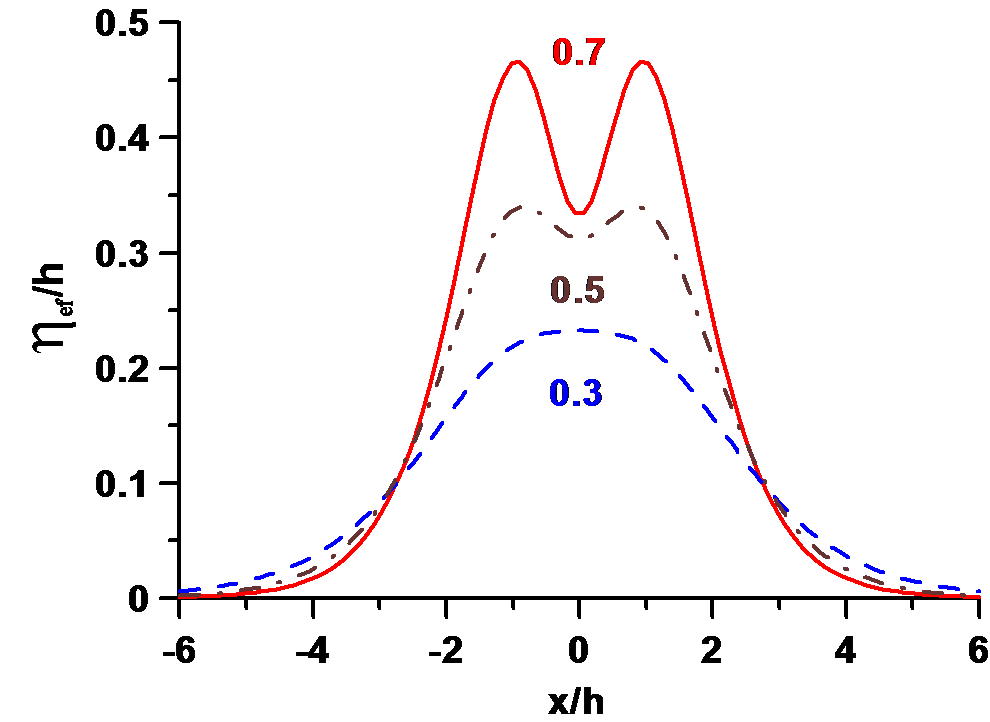
\includegraphics [width=0.7\linewidth] {solitonPress_3.png}
  \caption{Пространственное распределение донного давления, вызванное прохождением уединенной волны различной амплитуды $A/h$ (цифры на рисунке)}
  \label{img:solitonPress_3}
\end{figure}
\FloatBarrier



\section{Развитие и трансформация сильнонелинейного волнения в бассейне конечной глубины}

Для изучения развития сильнонелинейных процессов на поверхности жидкости в бассейне конечной глубины, был использован вычислительный комплекс....
%пару абзацев про комплекс
В качестве начальной волны задавалась волна Стокса (ссылка):
%описание волны-Стокса
\emph{(описание начальной волны Стокса)}

\begin{figure} [ht]
  \center
  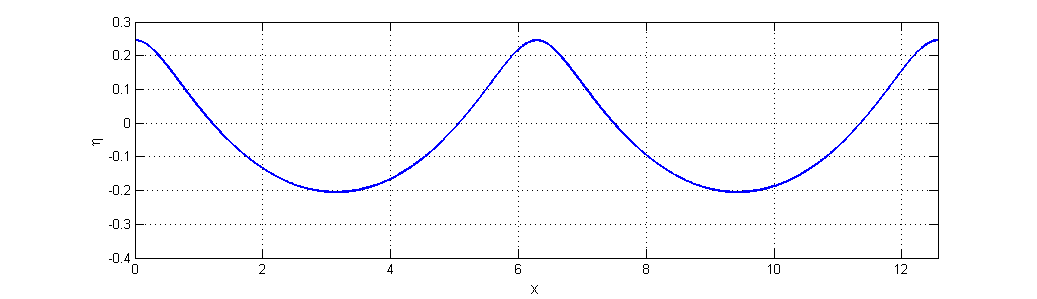
\includegraphics [width=170 mm] {res_1_w0.png}
  \caption{Профиль начальной стационарной волны}
  \label{img:res_1_w0}
\end{figure}
\FloatBarrier
На рис. \ref{img:res_1_w0} представлен профиль волны Стокса, задаваемой в качестве начального смещения поверхности.


Для изучения процесса обрушения волнения производилось несколько запусков одной и той же начальной волны Стокса с различной глубиной бассейна, принимающей значения
h=0.5, 0.7, 1, 1.5, 2, 3.
\begin{figure} [ht]
  \center
  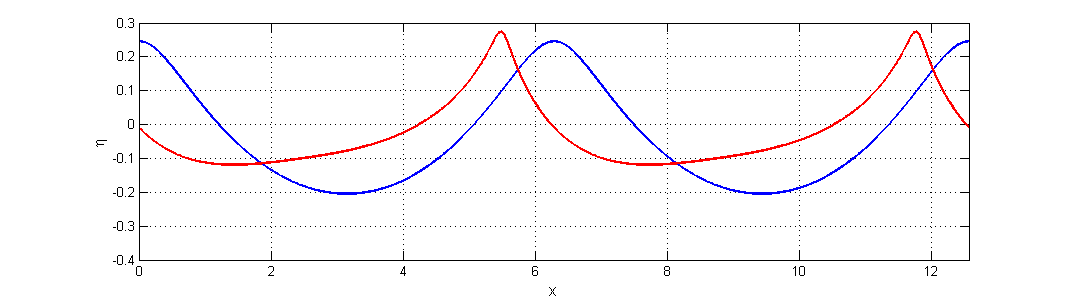
\includegraphics [width=170 mm] {res_1_w0_w40.png}
  \caption{Профили волны в начальный момент времени(синяя линия) и в момент обрушения волны.}
  \label{img:res_1_w0_w40}
\end{figure}
\FloatBarrier
На рис. \ref{img:res_1_w0_w40} сравниваются два профиля волны: в момент обрушения и в начальный момент времени. По графику видно как происходит укручение волны: волновой фронт становится практически перпендикулярным и волна становится сильно ассиметричной.

Для того, чтобы подробного изучения этого процесса, построим изменение максимальной крутизны волны от времени для различных глубин. Максимальная крутизна при этом рассчитывается по формуле
\begin{equation}\label{eq:steepnessPartial}
 C_{max}(t)=\max|\frac{\partial y(x,t)}{\partial x}|
\end{equation}


\begin{figure}[h]
\center
\begin{minipage}[h]{0.45\linewidth}
  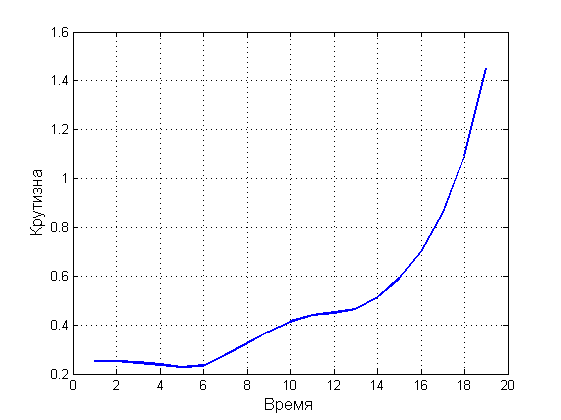
\includegraphics [width=1\linewidth] {res_05.png}
  \caption{Зависимость максимальной крутизны волны Стокса $C_{max}$ от времени, для глубины h=0.5}
  \label{img:res_05}
\end{minipage}
\hfill
\begin{minipage}[h]{0.45\linewidth}
  \center
  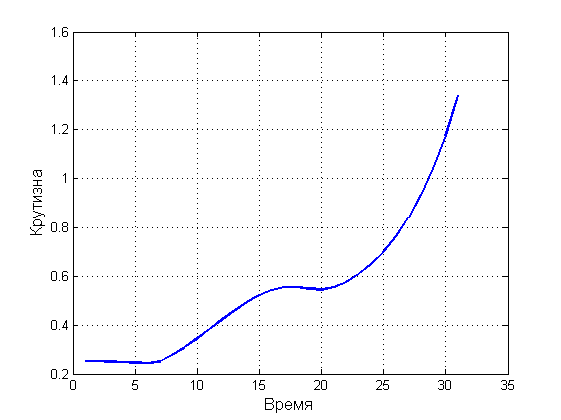
\includegraphics [width=1\linewidth] {res_07.png}
  \caption{Зависимость максимальной крутизны волны Стокса $C_{max}$ от времени, для глубины h=0.7}
  \label{img:res_07}
\end{minipage}
\end{figure}
\FloatBarrier

\begin{figure} [ht]
  \center
  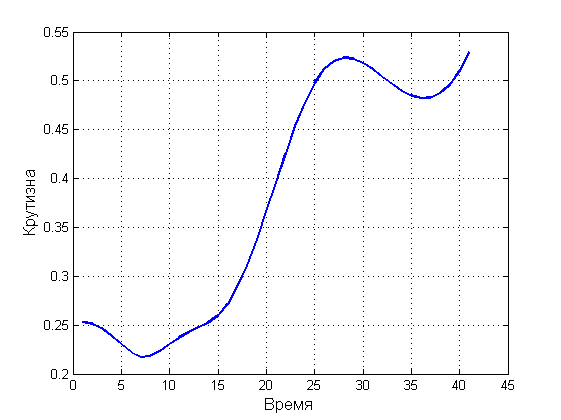
\includegraphics [width=0.5\linewidth] {res_1.png}
  \caption{Зависимость максимальной крутизны волны Стокса $C_{max}$ от времени, для глубины h=1}
  \label{img:res_1}
\end{figure}
\FloatBarrier
\begin{figure} [ht]
  \center
  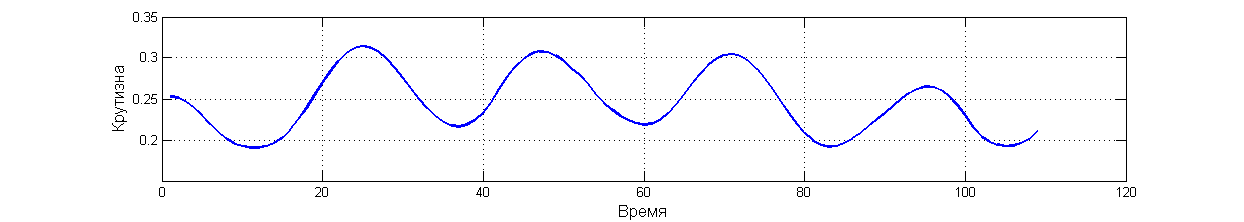
\includegraphics [width=1\linewidth] {res_1_5.png}
  \caption{Зависимость максимальной крутизны волны Стокса $C_{max}$ от времени, для глубины h=1.5}
  \label{img:res_1_5}
\end{figure}
\FloatBarrier
\begin{figure} [ht]
  \center
  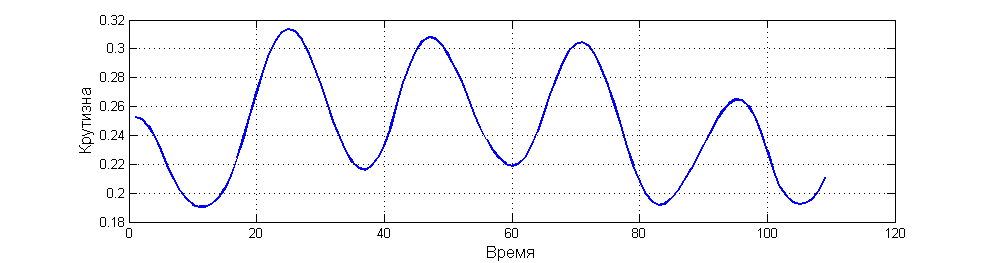
\includegraphics [width=1\linewidth] {res_2.png}
  \caption{Зависимость максимальной крутизны волны Стокса $C_{max}$ от времени, для глубины h=2}
  \label{img:res_2}
\end{figure}
\FloatBarrier
Как видно из рис.\ref{img:res_05}-\ref{img:res_2}, чем меньше глубина тем больше изменение крутизны со временем происходит по экспоненциальному закону. При б$\acute{о}$льших глубинах график изменения крутизны приобретает синосуидальную форму. И в некоторых случаях даже уменьшается.

Так же стоит отметить разную максимальную крутизну при которой наступает обрушение волны на различных глубинах.  Чтобы изучить подробнее этот факт построим график зависимости крутизны обрушения (или остановки счета)от глубины бассейна.

\begin{figure} [ht]
  \center
  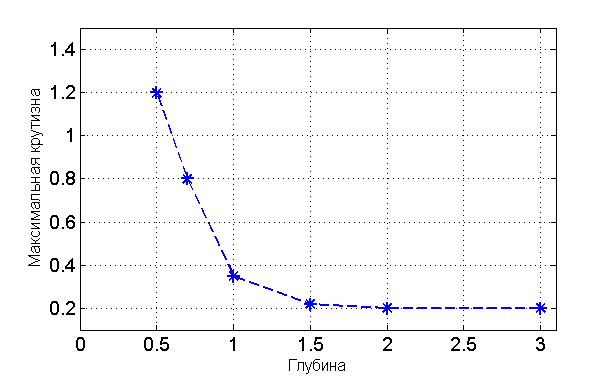
\includegraphics [width=1\linewidth] {Stepness_Depth.png}
  \caption{Зависимость крутизны обрушения волны Стокса от глубины}
  \label{img:Stepness_Depth}
\end{figure}
\FloatBarrier

Стоит отметить, что расчеты вынужденно остановились из-за разрушения схемы, т.е. в случае когда произошло обрушение волны только в случаях когда глубина бассейна была 0.5, 0.7 и 1. В случаях когда h=1.5, 2 расчеты продолжались до заданного времени расчета.

По графику \ref{img:Stepness_Depth} видно, что крутизна волны в конце расчетов изменялась в пределах от 1.2 до 0.2 таким образом. При этом обрушивалась волна при крутизне от 1.2 до 0.35, при $C_{max} = 0.2$. Таким образом можно сказать, что волна Стокса на мелководье может начинать обрушиваться при крутизне $0.2<C_{max}<0.35$ (крутизна рассчитывалась по формуле \eqref{eq:steepnessPartial}).

Также можно видеть, что график представленный на рис. \ref{img:Stepness_Depth} имеет экспоненциальную форму.


\section{Моделирование характеристик аномально больших волн.} \label{sect3_3}

\subsection{Энергетические и геометрические характеристики}
В вычислительных экспериментах рассматривается цуг волн периодический по пространственной переменой. При этом профиль свободной поверхности задается функцией $y=y(x,t)$, являющейся $2\pi$-периодической по переменной $x$.

В соответствии с (Шамин) без ограничения общности можно считать, что при всех фиксированных значениях переменной $t$ функция  является достаточно гладкой (существует не менее 2-х непрерывных производных по $x$) и имеет ровно N минимумов и N максимумов. Таким образом, мы имеем разбиение отрезка $[0,2\pi]$ на N подинтервалов:
$$
[0,2\pi]=\bigcup\limits_{i=1}^N[x_{i-1},x_i],
$$
где $x_i$ - точки минимумов, для простоты предположили, что в точке $x_0=0$ функция $y(x)$ имеет минимум. Таким образом, мы рассматриваем отдельную волну как область профиля заключенную между двумя локальными минимумами в фиксированный момент времени. Отдельную i-ую волну в профиле в фиксированный момент времени t будем называть $W_i(t)$. Для сокращения записи будем пользоваться обозначениями N и $W_i$.

Для каждой индивидуальной волны $W_i$ в профиле можно вычислить числовые характеристики.
Рассмотрим следующие характеристики (Шамин, Юдин):
\begin{enumerate}
  \item $\tilde{H}_i$ - высота, которая рассчитывается как
  $$
  \tilde{H}_i=\max_{x\subset[x_{i-1},x_i]}y(x)-\min_{x\subset[x_{i-1},x_i]}y(x),
  $$
  \item $\tilde{L}_i$ - длина волны, рассчитываемая как
  $$
  \tilde{L}_i=x_i-x_{i-1}
  $$
  \item $\tilde{M}_i$ - максимальная крутизна. Рассчитывается по следующей формуле
  $$
  \tilde{M}_i=\max_{x\subset[x_{i-1},x_i]}|\frac{\partial y(x,t)}{\partial x}|
  $$
  \item $\tilde{C}_i$ - максимальная кривизна, которая рассчитывается по следующей формуле:
      $$
  \tilde{C}_i=\max_{x\subset[x_{i-1},x_i]}\frac{|y_{xx}(x,t)|}{(1+y_x(x,t))^3/2}
  $$
  \item $\tilde{E}_i$ - полная энергия,
  \item $\tilde{T}_i$  - кинетическая энергия,
  \item $\tilde{U}_i$ - потенциальная энергия,
  \item $\tilde{I}_i$ - модуль импульса (состоящего из горизонтальной $\tilde{I}_i^{x}$ и вертикальной $\tilde{I}_i^{y}$ компонент).
\end{enumerate}

Энергия и импульс рассчитываются согласно формулам гидродинамики идеальной жидкости.

Для сравнительного анализа характеристик в различные моменты времени удобно использовать нормировку для характеристик отдельных волн. Покажем ее на примере характеристики $\tilde{C}_i$ - максимальной крутизны.

Отсортируем набор $\tilde{C}_i$ по возрастанию так, чтобы

$$
|\tilde{C}_1|<|\tilde{C}_2|<\ldots<|\tilde{C}_N|
$$

И обозначим его через $\hat{C}_i$. Далее построим нормированный набор величин

$$
C_i=\frac{N|\hat{C}_i|}{\sum\limits_{j=1}^{N}\hat{C}_j}
$$

Аналогично нормировка делается и для всех остальных 9-ти характеристик. Подобная нормировка позволяет проводить относительное сравнение набора характеристик в различные моменты времени, с учетом того что количество волн в оцениваемых профилях может быть различно.

Далее будут сравниваться графики описанных выше характеристик, рассчитанные в момент появления волны-убийцы и в начальный момент времени. В соответствии с (Шамин, Юдин) введем понятие концентрации характеристики в волне, как относительное превышение среднего значения характеристики в определенный момент времени.

Далее рассмотрим распределение концентрации характеристик на примере записей волн-убийц полученных в результате численных экспериментов.

\subsection{Пример распределения концентрации характеристик в момент образования волны-убийцы.}

Рассмотрим характерный пример формирования волны-убийцы. В данном эксперименте начальное поле волнения состояло из цуга 25 волн, бегущих в одну сторону. Квадрат средней крутизны принимал следующее значение $\mu^2 = 2.06*10^{-3}$, дисперсия D = 5. Длительность эксперимента составляла примерно 1000 периодов. Примерно через 913 периодов возникла волна-убийца.

\begin{figure} [h]
  \center
  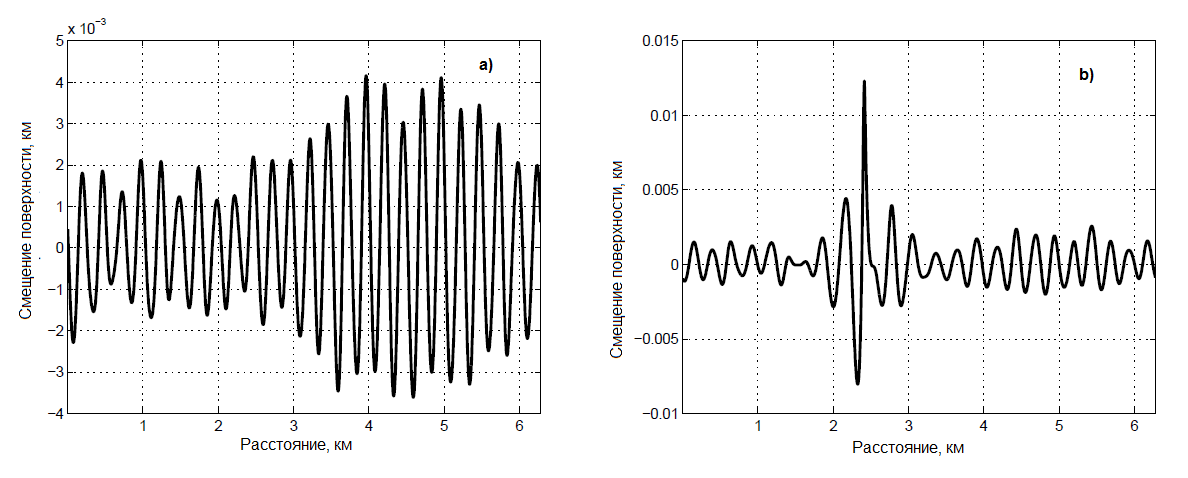
\includegraphics [width=170 mm] {profileNumFreak.png}
  \caption{Профиль поверхности жидкости в a) начальный момент времени b) в момент появления волны убийцы.}
  \label{img:profileNumFreak}
\end{figure}
\FloatBarrier

На рис. \ref{img:profileNumFreak}а приведен профиль начальной волны, через 913 секунд развития волнения возникла характерная аномально-большая волна, профиль которой показан на рис. \ref{img:profileNumFreak}b.

Возникшая волна-убийца обладает высотой превышающей значительную высоту волн в 3.14 раза.
$$
\nu=\frac{H_{max}}{H_S}=3.14
$$

Волна с таким отношением является крайне редко встречаемой и безусловно представляет из себя большую опасность ее можно назвать «сильной» волной-убийцей.  Известно, что процесс возникновения волн-убийц сопровождается концентрации большого количества энергии в этой волне. С помощью вычислительных экспериментов можно провести количественную оценку концентрации описанных выше характеристик.

Как видно из рис. \ref{img:allPict} на всех рассматриваемых характеристиках отмечается процесс концентрации ее в одной волне-убийце. Абсолютные значения концентрации характеристик (E, H, L, I, M, C) на этих графиках показывают во сколько раз энергия, высота, кривизна и т.д. i-ой волны превосходит среднее значение параметра волн в данный момент времени.

\begin{figure} [h]
  \center
  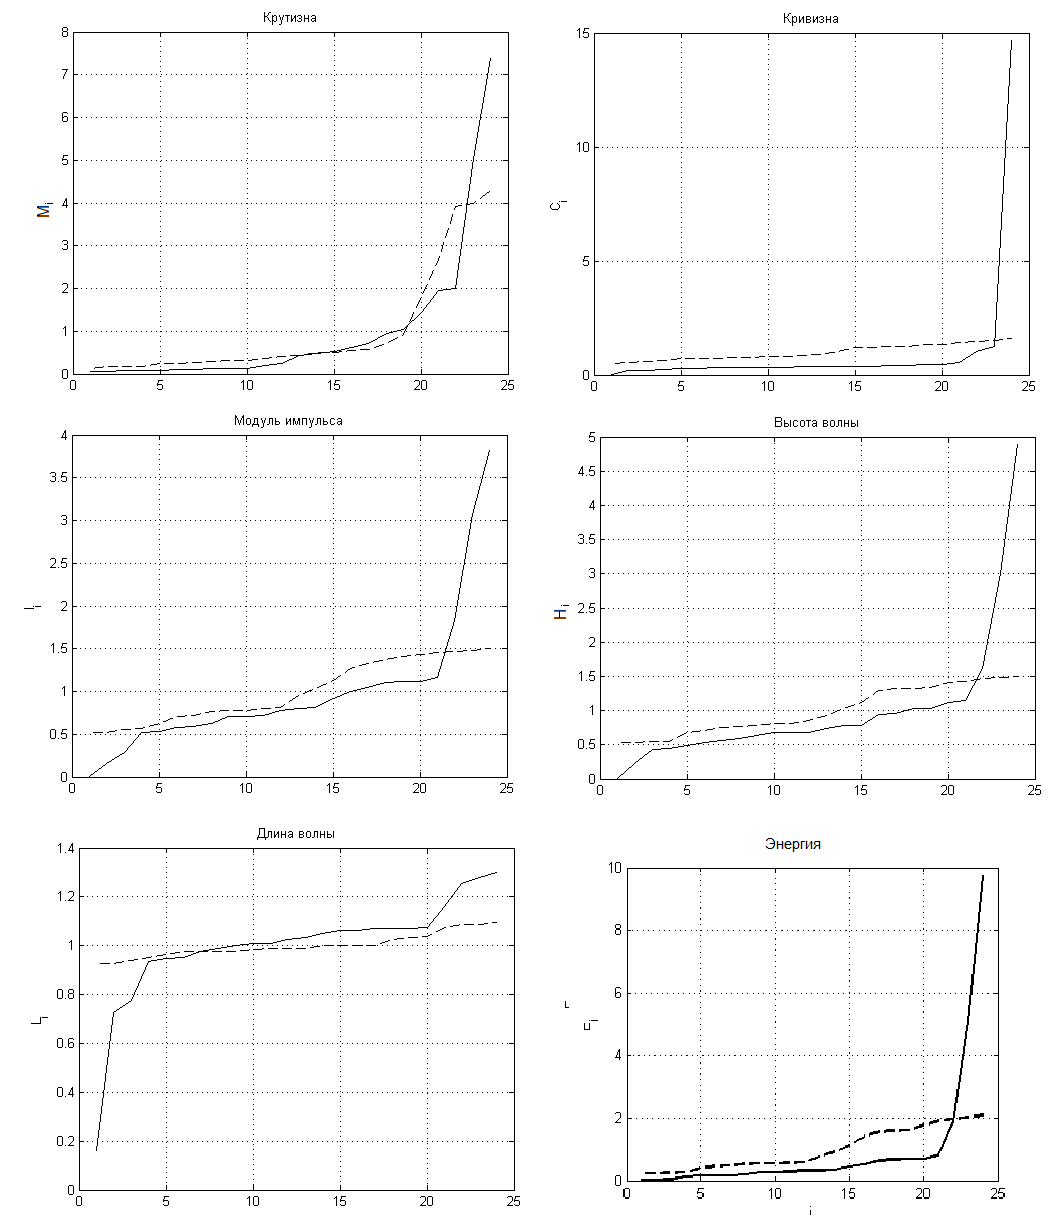
\includegraphics [width=170 mm] {allPict.png}
  \caption{Концентрация основных характеристик для  начального момента времени (пунктирная линия) и в момент появления волны-убийцы (сплошная линия)}
  \label{img:allPict}
\end{figure}
\FloatBarrier

Стоит отметить, что  длины волн распределяются существенно более равномерно, чем другие параметры (Шамин). Внести отклонения в это распределение может только такая сильная волна как рассматриваемая в этом примере.

Так же можно отметить, что некоторые параметры сильнее других реагируют на появление волны-убийцы, например такие как кривизна или полная энергия. А график концентрации других параметров в момент появления волны-убийцы практически не отличается от концентрации параметра в начальный момент, например, такой как крутизна.

Поэтому для выделения параметра, который лучше всего будет реагировать своим изменением на появление волны-убийцы, введем понятие степени чувствительности параметра. Данный параметр, будет описывать, то насколько чувствительна оцениваемая характеристика к наличию волны-убийцы.

\begin{equation}\label{eq:sensCoeff}
  s = \frac{max(X_{freak}) - min(X_{freak})}{max(X_{0}) - min(X_{0})}
\end{equation}

Анализ введенного параметра s позволит провести сравнительную оценку разных характеристик с различными абсолютными значениями и выделить среди них те, которые будут сильнее всего меняться при появлении волны-убийцы.

Рассмотрим пул экспериментов с различными начальными условиями. Начальное поле волнения состояло из цуга 25 волн, бегущих в одну сторону. Квадрат средней крутизны принимал значение $\mu^2$ от $2.06*10^{-3}$  до $5.02*10^{-3}$,   дисперсия D  от 1 до 25. Но основе пула вычислительных экспериментов состоящих из 23 событий волн-убийц, где параметр   варьировался от 2.11 до 3.14, рассчитаем диаграммы средних степеней чувствительности параметров и средние значения максимумов концентрации энергии, крутизны, кривизны, высоты и других параметров.
Диаграмма на рисунке 5 позволяет качественно оценить какая из перечисленных геометрических и динамических характеристик наиболее сильно меняется при появлении волны-убийцы.

\begin{figure} [h]
  \center
  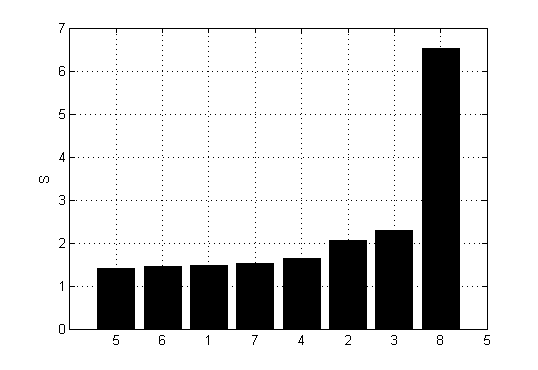
\includegraphics [scale=0.7] {Mean_S.png}
  \caption{Диаграмма средней степени чувствительности параметров $s$ на появление аномально-большой волны. (1) – Длина волны, (2) – Высота волны, (3) – Полная энергия, (4) – Модуль импульса, (5) – Горизонтальный импульс, (6) – Вертикальный импульс, (7) – Крутизна, (8) – Кривизна.}
  \label{img:Mean_S}
\end{figure}
\FloatBarrier



По рис. \ref{img:Mean_S} видно, что наиболее чувствительной характеристикой является кривизна. В среднем, она по своей чувствительности более чем в три раза превосходит другие параметры, такие как полную энергию и высоты волн. Меньше всего при появлении волны-убийцы меняются импульс (вертикальная и горизонтальная составляющие) и длина волны.




\section{Заключение} \label{sect3_0}
В данной главе обсуждается важная проблема восстановления параметров  ветровых волн по данным регистраторов давления, установленных на дне. В условиях достаточного мелкого моря процедура восстановления найдена с помощью слабодисперсионного обобщения нелинейной теории мелкой воды. В рамках негидростатической модели Железняка – Пелиновского, в которой учитывается произвольная нелинейность и слабая дисперсия, удается получить явное выражение для колебаний морской поверхности с использованием точечного измерения придонного давления. При этом используется однонаправленное приближение для ветровых волн с узким угловым спектром. Конкретные расчеты выполнены для условий Охотского моря, где на глубинах 5-20 м часто встречаются ветровые волны с периодами 4-7 секунд и амплитудами 10 - 40 см. Показано, что негидростатические поправки для почти монохроматических волн достаточно малы, что подтверждается также результатами лабораторного эксперимента, описанных в  \cite{Oliveras_2012}. В то же время негидростатические поправки оказываются существенными для импульсных сигналов, и могут достигать 50\%. Полученные формулы могут использоваться для анализа ветровых волн в мелководных районах морей и океанов.

Представлена формула затухания давления в рамках конформного представления уравнения Эйлера.

Произведены численные расчеты для сравнения линейной теории и полнонелинейной.

Возможно сравнение со слабодисперсионной полнонелинейной теорией.

В текущей главе на основе вычислительных экспериментов проведен количественный анализ процессов концентрации геометрических характеристик волн (длина, высота, крутизна, кривизна) и динамических (энергии и импульса) в момент образования аномально больших поверхностных волн, т.н. волн-убийц. Показано что наиболее чувствительными к аномально большой волне параметрами являются кривизна волны, энергия и высота. Т.е. при появлении волны-убийцы наиболее сильно меняются именно эти параметры.

Приведено соответствие этих результатов с данными натурного наблюдения аномально-больших волн на шельфе о.Сахалин.

Этот результат может быть использован при оценке риска опасного воздействия волн-убийц на суда и морские сооружения, поскольку показывает, что энергетические характеристики таких волн могут быть значительно выше, чем использующиеся значения в нормативных расчетах.



\clearpage
